% !TEX TS-program = pdflatex
% !TEX encoding = UTF-8 Unicode

% This is a simple template for a LaTeX document using the "article" class.
% See "book", "report", "letter" for other types of document.

\documentclass[11pt,twoside]{report} % use larger type; default would be 10pt

\linespread{1}
\renewcommand*\rmdefault{ptm}

\usepackage[utf8]{inputenc} % set input encoding (not needed with XeLaTeX)

%%% Examples of Article customizations
% These packages are optional, depending whether you want the features they provide.
% See the LaTeX Companion or other references for full information.

%%% PAGE DIMENSIONS
\usepackage{geometry} % to change the page dimensions
\geometry{a4paper} % or letterpaper (US) or a5paper or....
\geometry{
	margin=2.5cm,
} % for example, change the margins to 2 inches all round
% \geometry{landscape} % set up the page for landscape
%   read geometry.pdf for detailed page layout information

\usepackage{graphicx} % support the \includegraphics command and options

% \usepackage[parfill]{parskip} % Activate to begin paragraphs with an empty line rather than an indent

%%% PACKAGES
\usepackage{url}
\usepackage{booktabs} % for much better looking tables
\usepackage{array} % for better arrays (eg matrices) in maths
\usepackage{paralist} % very flexible & customisable lists (eg. enumerate/itemize, etc.)
\usepackage{verbatim} % adds environment for commenting out blocks of text & for better verbatim
\usepackage{subfig} % make it possible to include more than one captioned figure/table in a single float
\usepackage[final]{pdfpages}
% These packages are all incorporated in the memoir class to one degree or another...

%%% HEADERS & FOOTERS
\usepackage{fancyhdr} % This should be set AFTER setting up the page geometry
\pagestyle{fancy} % options: empty , plain , fancy
\renewcommand{\headrulewidth}{0pt} % customise the layout...
\lhead{\small Teaching Quantum Mechanics Using qCraft}\chead{}\rhead{\small Micha van den Enk, s1004654}
\lfoot[\small \today]{\small \thepage}
\cfoot{}
\rfoot[\small \thepage]{\small \today}

%%% SECTION TITLE APPEARANCE
\usepackage{sectsty}
\allsectionsfont{\sffamily\mdseries\upshape} % (See the fntguide.pdf for font help)
% (This matches ConTeXt defaults)

%%% RULE

\newcommand{\HRule}{\rule{\linewidth}{0.5mm}}

%%% BIBLIOGRAPHY

\usepackage{apacite}                           %bibliography in apa-style

%%% ToC (table of contents) APPEARANCE
\usepackage[nottoc,notlof,notlot]{tocbibind} % Put the bibliography in the ToC
\usepackage[titles,subfigure]{tocloft} % Alter the style of the Table of Contents
\renewcommand{\cftsecfont}{\rmfamily\mdseries\upshape}
\renewcommand{\cftsecpagefont}{\rmfamily\mdseries\upshape} % No bold!

\setcounter{secnumdepth}{-2}

%%% TABLES

\renewcommand{\arraystretch}{1.2}

\usepackage{afterpage}

\newcommand\blankpage{%
    \null
    \thispagestyle{empty}%
    \newpage}

%%% END Article customizations

%%% The "real" document content comes below...

\begin{document}

\begin{titlepage}

\begin{center}


% Upper part of the page

\includegraphics[width=1\textwidth]{./logo}\\[1cm]    

\textsc{\Large Bachelor Thesis}\\[0.5cm]
\textsc{\Large {[}201000166{]}}\\[0.5cm]


% Title
\HRule \\[0.4cm]
{ \huge \bfseries Teaching Quantum Mechanics Using qCraft}\\[0.4cm]

\HRule \\[1.5cm]

% Author and supervisor
\begin{minipage}{0.4\textwidth}
\begin{flushleft} \large
\emph{Author:}\\
Michaël Christiaan \textsc{van den Enk} \\
{[}s1004654{]} \\
\end{flushleft}
\end{minipage}
\begin{minipage}{0.4\textwidth}
\begin{flushright} \large
\emph{Supervisors:} \\
Dr. H. H. \textsc{Leemkuil} \\
Dr. H. \textsc{van der Meij} \\
\end{flushright}
\end{minipage}

\vfill

% Bottom of the page
{\large \today}

\end{center}

\end{titlepage}

\afterpage{\blankpage}

\setcounter{tocdepth}{1}
\tableofcontents
\thispagestyle{fancy}
\newpage

\section{Preface}

%%% ANALYSIS

\subsection{The Generic Model}

\begin{figure}[h]
\centering
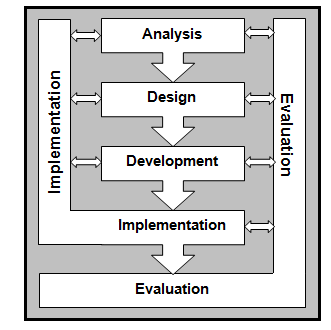
\includegraphics[width=0.7\textwidth]{genericmodel}
\caption{The generic model by \protect\citeA{genericmodel}\label{fig:genericmodel}}
\end{figure}

\subsection{Topics mentioned in literature}
\label{sssec:topicsliterature}

The first logical question which should be asked would be the question which topics exist within the domain of introductory quantum mechanics, because only then we can delve into the question how these topics could or should be thought to novice learners. This exploration would have to start with a topic the students are already familiar with. Such a topic is the Rutherford-Bohr Model of the Atom, also known as the Bohr Model, which presents a description of a hydrogen atom (see figure~\ref{fig:bohrmodel}). Students in upper secondary education should at least be familiar with this model, especially those with a technical profile. This gives way to introduce the students to the concept of elementary particles, which are the particles which exhibit quantum behaviour. The Bohr-model is also often referred to in the studied literature \cite{dori, mckagan, muller, papaphotis1, papaphotis2}.

\begin{figure}[h!]
\centering
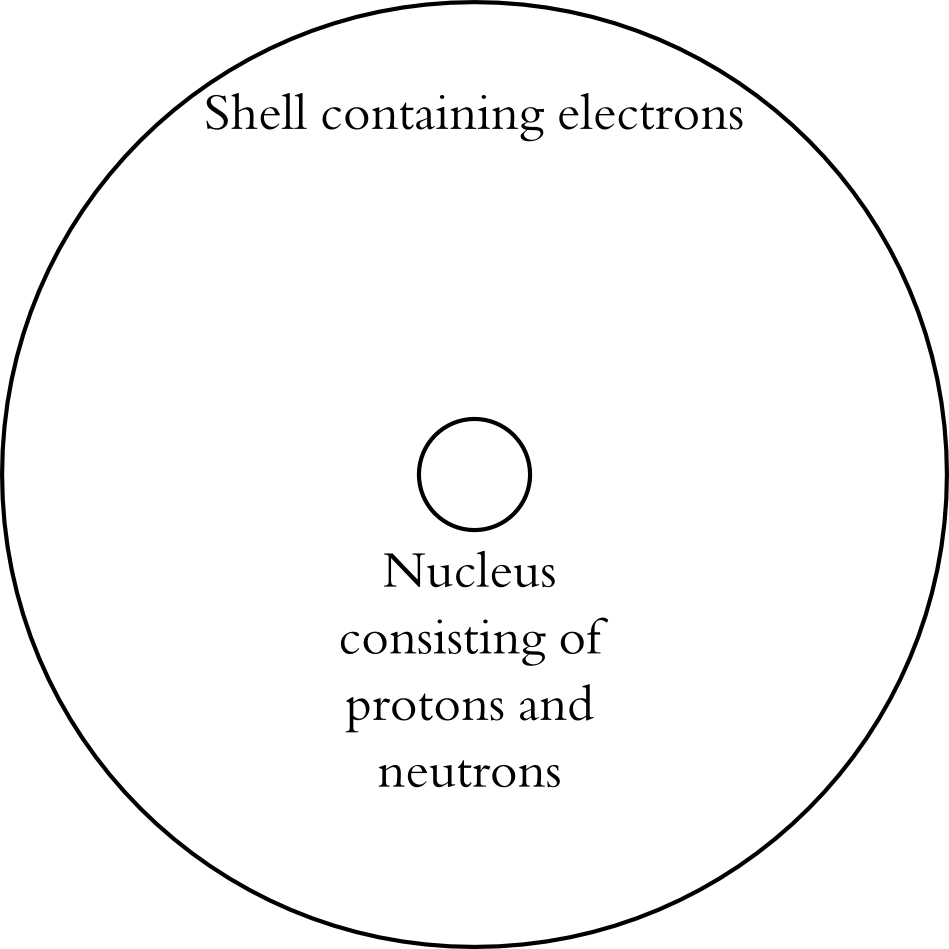
\includegraphics[width=0.5\textwidth]{bohrmodel}
\caption{The Rutherford-Borh Model of the Atom}
\label{fig:bohrmodel}
\end{figure}

Some of the studies \cite{erduran, hubber, muller, thacker} then describe properties of specific elementary particles, mostly of electrons or photons. Often used properties are the photoelectric effect or the polarisation of light \cite{henriksen, mckagan, muller}. These properties could give more meaning to what the elementary particles are and do. Another benefit would be that these properties are used in the various experiments conducted within the field of quantum mechanics.

The double-slit experiment is the most famous of these experiments, and also the most studied tool for educational purposes \cite{asikainen, henriksen, hobson, levrini, mckagan, muller, papaphotis1,singh2, thacker}. A reason why this experiment is famous is because it was the first experiment in history to demonstrate phenomena of quantum mechanics. The experiment entails shooting elementary particles through two narrow slits in a wall, projecting them on a large wall behind these two slits. When the two slits are separated very little, a interference pattern emerges. This is a result expected when the elementary particles would not be particles but waves. However, if the particles are observed and information is available through which slit each particle traversed, a diffraction pattern emerges, which would be the behaviour of particles. The most apparent phenomena demonstrated by this experiment is the wave-particle duality of elementary particles, which then could give way to mathematical descriptions of quantum mechanics like the Schrödinger equation. The Centraal Eindexamen of 2015 also already contained this experiment \cite{eindexamen2015}, so educational resources for teaching this experiment already exist.

For understanding the double-split experiment, the concept of superposition is vital. Superposition means that when a particle is not observed, it is in all possible states at the same time. In the case of the double-slit experiment, superposition means that the particle goes through both slits at the same time. It then interferes with itself because of the probability function of where the particle ends up. However, when the particle is observed through which slit it travels, the information through which slit the particle travels is known and forces the probability function of the particle to collapse to either the left or the right slit. Because of this, it behaves like a particle and a diffraction pattern emerges. A video which demonstrates the double-slit experiment can be seen on \url{https://upload.wikimedia.org/wikipedia/commons/transcoded/e/e4/Wave-particle_duality.ogv/Wave-particle_duality.ogv.480p.webm}. The double-slit experiment can provide the learner with an explanation of the observer dependency of the elementary particles. However, only \citeA{muller} mentions this concept in his study, and it also does not appear in the Centraal Eindexamen of 2016 \cite{eindexamen2016}.

The concept of superposition also has different cases. There are other properties of elementary particles which can be in superposition, for example the polarity of photons. Upon measurement, the polarisation value of a photon particle collapses to a certain value, but before this collapse it has all the different polarities at the same time. This gives way to the concept of entanglement, mentioned in some studies \cite{henriksen, hobson, kuttner}. Entanglement is a phenomenon which occurs between elementary particles, and it has as effect that the collapse of the different particles are interdependent of each other. This entanglement has two forms: boson entanglement and fermion entanglement. When the two particles are bosons, they always collapse to the same state on observation, and when the two particles are fermions, they always collapse to each others opposite state.

Since the discovery of the phenomena occurring within quantum mechanics, scientists have debated fiercely about how to interpret these phenomena \cite{barnes}. Roughly speaking, the scientists could be divided intro two camps: the camp of the realists and the camp of the ontologists. The realists thought that there has to be something underneath quantum mechanics which could explain the strange phenomena of superposition and entanglement, whereas the ontologists thought that the phenomena of quantum mechanics stand on its own. The phenomena of entanglement played a huge role in this debate. The realists first thought that they could use entanglement to prove that there is a reality underneath quantum mechanics, but it eventually led mostly to evidence towards the camp of ontologists. One example of this is Bell's inequalities \cite{kuttner, muller}, which is beyond the scope of this literature study to explain.

\citeA{henriksen} writes that there are three main differences between classical mechanics and quantum mechanics. The first difference is the fact that classical mechanics are deterministic and that quantum mechanics are probabilistic, also brought up by \citeA{levrini} and by \citeA{papaphotis1}. Classical mechanics rely heavily on deterministic causal effects, which can ultimately be explained. This is very apparent in systems of force, where everything moves according to certain laws, take for example the three Newtonian laws. Quantum mechanics however relies heavily on probabilistic models, where certain properties of certain elementary particles collapse to certain values according to probability functions.

A second difference between classical mechanics and quantum mechanics mentioned by \citeA{henriksen} is the locality of classical mechanics and the non-locality of quantum mechanics, also mentioned by \citeA{hobson}. On the scale of classical mechanics, it is possible to determine the exact position of an object, at least it is possible to do this on a significant scale. On a very small scale however, on the scale of quantum mechanics, the exact position of an object  cannot be determined. There is an inherent uncertainty about the position of an object, which is very small and insignificant on the scale of classical mechanics, but quite significant on the scale of elementary particles. This is also true for the momentum of an elementary particle, which can be translated to the speed of an elementary particle. This uncertainty can be demonstrated by the uncertainty principle of Heisenberg \cite{henriksen, muller, velentzas}, which has as implications that neither the location nor the momentum of an elementary particle can be exactly known and that the more certain the location of an elementary particle is known, the less certain the momentum of an elementary particle can be known and vice versa.

Finally, \citeA{henriksen} mentions that classical mechanics are continuous and that quantum mechanics are discrete. This is because of the Planck length, which is the shortest measurable length. In classical mechanics, this length is very insignificant, and because of that the world looks continuous. A fully continuous world would mean that there is no tiniest unit, but that it is always possible to “go smaller”. For example, if one had a plank of wood, it could be divided in half infinitesimally. However, on a quantum scale, this is not possible, because it is not possible to have something smaller than the Planck length.

Because of the inherent difficulty with quantum mechanics, some scientists have posited thought experiments, which allows the learner to make a mental model about the different concepts of quantum mechanics. The most famous thought experiment is that of Schrödinger's cat \cite{muller, velentzas}, where the life of a cat depends on the collapse of an elementary particle. When the cat is then observed, the state of the elementary is observed indirectly, which causes it to collapse and either kill the cat or let the cat live. This teaches the student about observer dependency, the way observations are linked to the random collapse of an elementary particle. Another thought experiment mentioned in the studied literature is the EPR paradox \cite{kuttner, muller, velentzas}, which can be used to teach the student about how entanglement is related to deep questions about the nature of quantum mechanics. This thought experiment however is related to the EPR experiment, which lies beyond the scope of this study to explain.

Finally, there are some studies which recommend certain mathematical approaches to quantum mechanics, namely the Schrödinger's equation \cite{muller, singh2}, the Hermitian operator \cite{singh2}, the aforementioned Bell's inequalities \cite{kuttner, muller}, the eigenvalue equation \cite{muller} and the DeBroglie energy levels \cite{dori, gianino, mckagan}. However, these mathematical approaches rely on a thorough conceptual understanding of quantum mechanics and are therefore not relevant to this study.

The topics relevant to teaching quantum mechanics can be summed up as the Rutherford-Bohr model of the Atom and elementary particles, the double-slit experiment, superposition, entanglement, the debate between realists and ontologists, the differences with classical mechanics, thought experiment and the mathematical side of quantum mechanics.

\chapter{Analyses}
\thispagestyle{fancy}

The first step of the Generic Model by \citeA{genericmodel} (see figure~\ref{fig:genericmodel} on page~\pageref{fig:genericmodel}) is Analysis. \citeA{smithragan} give an elaborated description of how to perform these analyses for instructional design. They distinguish three different kinds of analysis: analysing the learner context, analysing the learner and analysing the learning task. The analysis of the learning context can provide the instructional needs and a description of the different factors influencing the instruction. The purpose of the learner analysis is the characterisation of the end user of the instruction, which is in this case the middle school students. Conducting a context analysis and a learner analysis is also in concurrence with the Generic Model, which states that from the very beginning in the analysis phase the designer should already start with the implementation of the instruction \cite{genericmodel}. In the task analysis the test specifications are written, with which the content of the instruction can be established.These three analyses are executed in the following three sections. As also can be seen in the Generic Model, it is important to start with evaluating the product already in the analysis phase. Therefore, the final section of this chapter describes the evaluation of the test specifications with an expert.

% Context Analysis

\section{Context Analysis}

A learning task always takes place in a certain learning context. In this case this is the middle school. It entails not only the place, but also the temporal and social environment \cite{smithragan}. The analysis of the learning context can provide the instructional needs and a description of the different factors influencing the instruction. With the instructional needs, the designer can establish the main learning goals for the instruction. The description of the learning environment can provide the learning opportunities and constraints which have to be taken into account for the instruction.

%needs assessment

\subsection{Needs Assessment}

The first goal of the need assessment is to investigate whether there exists a need for the instruction.  Without a need, it would be a waste of resources to develop the instruction \cite{smithragan}. Next to this, it is conducted to better specify the need for the instruction. In the context of instruction, the assessment often results in a learning goal, which is the main goal of the instruction. This main goal is needed to continue the rest of the analyses, because all other analyses are conducted in respect to this goal. The goal can also be used to construct the summative evaluation, because when this goal is achieved, the instruction has proved to be successful.

\citeA{smithragan} identify three different models for the needs assessment, namely the problem model, the innovation model and the discrepancy model (see figure~\ref{fig:needsassessment}). The problem model is used when there exists a problem in the current system which has to be solved. As can be seen in figure~\ref{fig:needsassessment}, this model is to be used as a prerequisite for the other two models for assessment. With this model, it is determined whether there really is a problem, whether the cause of the problem is related to the performance of employees or to the achievement of learners, whether the solution to the problem is learning and whether instruction for these learning goals is currently offered. After the problem model, the needs assessment splits into the two other models. The innovation model is used when there is a new learning goal that the learners should achieve, and the discrepancy model is used when the already available instruction is not adequate to achieve the learning goal. The designer should choose one of these models for his needs assessment.

\begin{figure}[h]
\centering
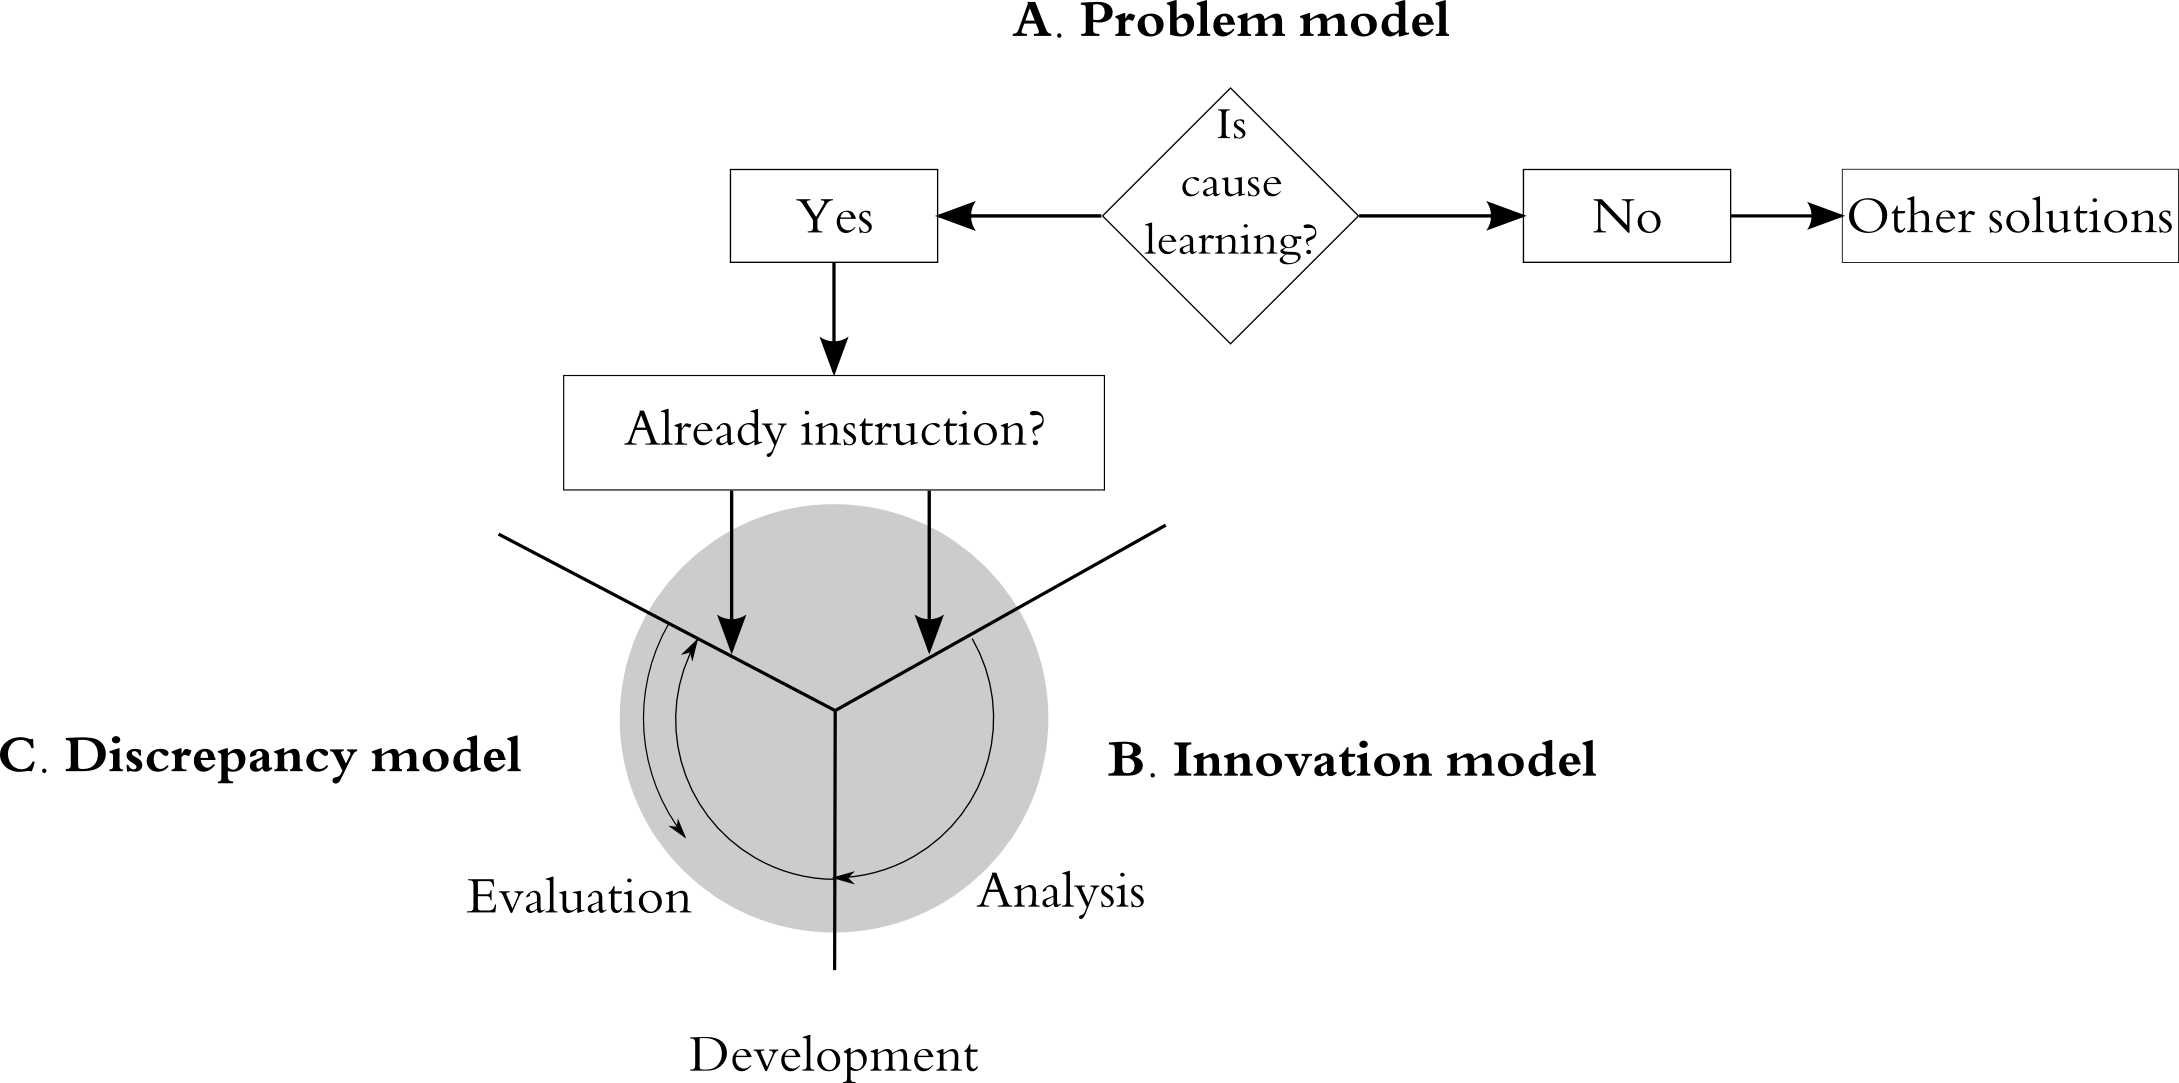
\includegraphics[width=\textwidth]{needsassessment}
\caption{The three sides of needs assessment \protect\cite{smithragan}\label{fig:needsassessment}}
\end{figure}

In the case of the instruction which will be constructed for this assignment, at first the problem model will be used to investigate the problem, and which of the two follow-up models should be used for the needs assessment.

\subsubsection{The problem}
\label{sssec:problem}

In the Netherlands, quantum mechanics always used to be a topic which schools themselves could choose to teach or not to teach. The only skill students had to know for the Centraal Eindexamen (the national central exams at the end of high school) which comes close to quantum mechanics is to elucidate the photoelectric effect and the wave-particle duality, mentioned within point 20 under subdomain E3 \cite{eindexamen2015}. However, one of the changes in the Centraal Eindexamen of 2016 was the addition of domain F1, which is called Quantum world \cite{eindexamen2016}. For this subdomain the candidate has to be able to apply the wave-particle duality and the uncertainty principle of Heisenberg, and to explain the quantization of energy levels in some examples with a simple quantum physical model. In order to give all candidates a chance of passing this subdomain, schools have to alter their programs in order to meet the expectations of the Centraal Eindexamen.

However, when searching the internet using the search machine Google concerning the implementation of quantum mechanics in Dutch high schools, the quantity and the quality of the results are very low. There are also no results to be found in the Dutch papers. An example is the Dutch site http://www.quantumuniverse.nl/, where teachers can find a small amount of brief courses on fundamental quantum mechanics, and where the forums are very quiet with only 5 discussions, of which 4 are just started threads from the site administrator.

Upon finding this information, an expert was consulted to confirm this conjecture. The expert was researching the implementation of quantum mechanics on in Dutch secondary education, and she also a first degree physics teacher. She stated that within her school there were no initiatives to bring this topic in their classrooms, and that their school was no exception as well.

The fact that next year domain F1 has to be fully implemented and taught to all vwo students who chose physics as an examination subject is therefore slowly turning into a sword of Damocles. This stresses the urgency for the development of new course material. This is an example of extrinsic motivation. However, is there also intrinsic motivation to teach quantum mechanics on high schools? First of all, there is no article which claimed that quantum mechanics should not be taught on high schools. On the other hand there are but a few authors who did have some arguments in favour of teaching. \citeA{muller} and \citeA{henriksen} state that quantum mechanics shapes our world view and that educated citizens should therefore become acquainted with the topic. It is also regarded as fundamental and should therefore be taught \cite{henriksen,hobson}. Finally, \citeA{erduran} states that the teaching of philosophical themes in science education has been advocated for several decades, and quantum mechanics is one of these themes.

Because it involves new instruction, the innovation model will be used for the second part of this needs assessment.

\subsubsection{The innovation}
\label{sssec:needsassessmentinnovation}

The nature of the innovation lies within the change of the Centraal Eindexamen of 2016 in respect to the Centraal Eindexamen of 2015. The new additions within the domain Kwantumwereld outline the new goals of physics education in the Netherlands, and will be the ultimate goals for the students to achieve, and therefore be the ultimate learning goals for the students to achieve. This results in the following learning goals \cite{eindexamen2016}:

The candidate can:
\begin{itemize}
\item describe quantum phenomena in terms of the enclosure of a particle:
\begin{itemize}
\item estimate whether quantum phenomena are to expected by comparing the debroglie-wavelength with the order of largeness of the enclosure of the particle;
\item apply the uncertainty principle of Heisenberg;
\item describe the quantum model of the hydrogen atom and calculate the possible energies of the hydrogen atom;
\item describe the quantum model of a particle in a one-dimensional energy well and calculate the possible energies of the particle;
\item Bohr radius, zero-point energy.
\end{itemize}
\item describe the quantum-tunnel effect with a simple model and indicate how the chance of tunneling depends on the mass of the particle and the height and width of the energy-barrier,
\begin{itemize}
\item minimal in the contexts of: Scanning Tunneling Microscope, alpha-decay.
\end{itemize} 
\end{itemize}

These goals confirm what the literature describes about the current appliance of quantum mechanics teaching within secondary, namely that often quantum mechanics is introduced with great emphasis on learning and practising algorithmic skills \cite{papaphotis1,papaphotis2}. However, it is also found that high school students show higher interest in the conceptual aspects than the algorithmic aspects \cite{papaphotis1,papaphotis2,levrini}. When focusing on the conceptual aspects, it engages students \cite{henriksen} and students start asking fundamental questions \cite{mckagan}. Furthermore, mathematical oriented approaches might be more common, however, quantum mechanics is regarded to be mathematically challenging \cite{gianino, mckagan}, and most high school students lack proper background in mathematics at the required level \cite{dori}. Because the usual focus on the algorithmic aspects, students often do not learn what instructors want them to learn \cite{asikainen, mckagan}, and improved student learning is possible by shifting the focus to conceptual understanding \cite{mckagan}.

Therefore, the aim of this instruction is to focus on a conceptual approach instead of a mathematical approach. Then, after the students have a sufficiently conceptual understanding of the material, the concurrent instructions in the curriculum can emphasise the goals stated by the Centraal Eindexamen of 2016, which adds the mathematical layer on top of the conceptual layer and can deepen the understanding of quantum mechanics. In summary, the main goal of this instruction is \emph{to provide the student with a conceptual understanding of the different phenomena occurring in the realm of quantum mechanics}.

%learning environment

\subsection{Learning Environment}

The learning environment description is the other major component of the learning context analysis \cite{smithragan}. The description contains information of all the external factors influencing the instruction. These are the mediators of the instruction, the already existing curricula which takes place in the environment, the available equipment available on the location of the instruction, the characteristics of the facilities at the location of the instruction, the characteristics of the organisation in which the instruction will take place, and the philosophies and taboos of the larger community in which this organisation exists.

A current first degree teacher training \cite{leraarnatuurkundemaster} does encompass quantum mechanics, so teachers which had this training should be familiar to the domain. However, \citeA{asikainen} states that teachers often still possess misconceptions about quantum mechanics, which are comparable to the misconceptions of the students themselves. These misconceptions will be discussed in the learner analysis section on page~\pageref{sec:learneranalysis}. Experienced teachers who are teaching modern physics are more capable of teaching quantum mechanics \cite{asikainen}.

When implementing the instruction, the placing within the already existing curriculum is also important, because the instruction depends on prerequisites from other elements of the curriculum. The main prerequisite is knowledge of Bohr his atom model, because the different particles within this model are the particles on which quantum mechanics apply. This knowledge is taught in Domain E from the centraal eindexamen \cite{eindexamen2016}, and because of the prerequisite, it is of upmost importance that this instruction is placed after Domain E in the existing curriculum. As already described in the needs assessment, the conceptual instruction could be followed by instruction of the mathematical aspects of quantum mechanics. Also, various experiments could be taught, which demonstrate the discovery of the various concepts introduced in the instruction and explain the different principles between the concepts. This could for example be the EPR experiment \cite{kuttner, muller, velentzas}, which could lead to critical assessment of the realist and ontologist perceptions on quantum mechanics.

Another important aspect of the instructional environment is the method of delivery \cite{smithragan}. The recommendations for different aspects of the medium used for the delivery of the instruction entail interactivity, visualisation, the combination of different modes of representation, and the use of computation. By making it able to interact with the medium, it is possible for students to experiment with the different concepts, which gives way to inquiry learning \cite{adegoke, asikainen, dori, mckagan}. Visualisation is a powerful tool, and can make the matter less abstract \cite{dori, henriksen, mckagan}. It also is easier to build mental models of quantum mechanics. \citeA{levrini} warns however against the use of oversimplified visualisations, because pictures are extremely partial and can be misleading. Therefore, it is important that the visualisation does not entail any unnecessary simplified representation of the matter. This combined with other different modes of representation, for example a textual description of the concept, makes it possible for the student to complete their mental model \cite{dori}. Finally, the use of computation makes it possible to take away the mathematical complexity from quantum mechanics, making way for a purely conceptual approach \cite{barnes, mckagan, velentzas}.

One could combine all these aspects by using simulations, which is also recommended by \citeA{mckagan}. However, teachers often prefer traditional lectures, because that is easier to implement in their classroom \cite{adegoke}. This difficulty has to be overcome if quantum mechanics is to be implemented successfully in the classroom. Furthermore, it has to be investigated whether the sufficient hardware is available in the learning environment.

Finally, it is important to investigate whether the instruction fits in with the mission and vision of the school, and also the philosophies and taboos that the teachers hold. Therefore, it is advised to find these discrepancies by the means of interviews, in which the school board is asked about their mission and vision, and the teachers about their personal believes in regard to quantum mechanics.

In any case, this assignment does not look into the implementation of the instruction yet, so these factors have to be looked closer at when embedding the instruction in the context of a specific school.

% Learner analysis

\section{Learner Analysis}
\label{sec:learneranalysis}

The second analysis is that of the learners \cite{smithragan}. The purpose of this analysis is the characterisation of the end user of the instruction, which is in this case the students of secondary education in the Netherlands, mostly ranging from age 17 to 18. This analysis will focus itself on the general misconceptions held by members of this demographic.

When developing an instruction, it is important to consider the already available conceptions on the topic. In quantum mechanics, these preconceived models often prove to be incorrect \cite{asikainen, papaphotis2, thacker}. This partly comes from the nature of quantum theory \cite{papaphotis2}, but also partly from textbooks and instruction \cite{hubber, papaphotis2}. The problems often stem from depending on outdated deterministic or realist models \cite{hubber, papaphotis1, papaphotis2}, an often mentioned example of this is that students often mix up the deterministic planetary model with the indeterministic atom model \cite{dori, henriksen, hubber, muller, papaphotis1, papaphotis2}. \citeA{mckagan} also mentions that it is difficult for students to recognise the scale in which quantum mechanics take place.

\citeA{thacker} describes how much knowledge of students consists out of memorised facts, for example that light is a wave and electrons are particles. When the student then is confronted with new or different information from what they know, they develop new memorised facts instead of creating the right model. This then results in models consistent with fragmented models of microscopic processes, which are often incorrect but self-consistent with a certain experiment \cite{hubber, thacker}. When the student cannot model the fragments anymore, this can result in deep skepticism towards quantum mechanics \cite{barnes, henriksen, levrini}. \citeA{muller} has created a long list of exact conceptions students hold about microscopic phenomena, which are too detailed to enlist fully in this article.

The misconceptions described in the studied articles mostly are measured in relation to the teaching material which is currently employed within schools or universities. This material is already described in the preface, and can generally described as misconceptions in relation to the Rutherford-Bohr model of the atom, and in relation to experiments like the double-slit experiment. However, it would be interesting to investigate the misconceptions in relation to the fundamental concepts of quantum mechanics themselves, for example in relation to elementary particles, superposition, random collapse of the probability function and entanglement. This would give greater insight in the conceptual understanding of students. However, no research has been conducted in these areas yet.

% Task analysis

\section{Task Analysis}

The final step is analysing the learning task \cite{smithragan}. In this analysis the goals from the needs assessment during the analysis of the learning context have to be translated to test specifications, with which the content of the instruction can be established. To establish these test specifications, it is important to investigate the learning goal first. This will be followed by a description of the various strategies mentioned within the literature for how to teach quantum mechanics. The next step is the prerequisite analysis, which is a description of the prerequisite knowledge the students have to possess in order to partake in this instruction in relation to the content, described in the section \emph{Topics mentioned in literature} on page~\pageref{sssec:topicsliterature}. After that, the learning objectives can be written, which model the outline of the instruction. Finally, the test specifications are formulated, which can be used to measure the student his understanding of quantum mechanics after the instruction.

\subsection{Learning goal}

The main learning goal as specified needs assessment using the innovation model from page~\pageref{sssec:needsassessmentinnovation}, the instruction will pursue provide the student with a conceptual understanding of the different phenomena occurring in the realm of quantum mechanics. This goal will be the main guideline for the information-processing analysis. However, it will not be possible to provide the students with a complete conceptual understanding of quantum mechanics. First of all, not even the scientific community has a full grasp of quantum mechanics, because it is a relatively new and still developing subject area. Second to that, physics students in secondary education do not have the time needed to gain at least the complete conceptual understanding of quantum mechanics available from the scientific community. Finally, there is not enough time to design an instruction which achieves a complete conceptual understanding, and the time available for this instruction is also limited. Therefore a choice has to be made in the different topics being taught.

Furthermore, there exists a consensus within the studied articles that quantum mechanics is a difficult topic, and this is also a consensus among educators \cite{gianino,papaphotis1,papaphotis2}. There are a couple of reasons mentioned within the articles to explain this topical difficulty. A couple of sources state that quantum mechanics is a very counter intuitive topic \cite{henriksen, levrini, mckagan, singh2}, because it contradicts many aspects of our daily experience, like locality or determinism. Quantum mechanics is also considered to be a very abstract topic \cite{barnes, gianino, mckagan, papaphotis1, singh1}. Because quantum mechanics differs a lot from our everyday experiences and because of its abstractness, it is difficult for learners to visualise the concepts of quantum mechanics \cite{henriksen, mckagan}. Another factor contributing to the difficulty of quantum mechanics is that it is mathematically challenging \cite{gianino, mckagan}, it involves mathematical skills that most high school students --- even vwo 6 students --- do not possess. Because of the difficulties stemming from teaching quantum mechanics, it would be better to teach concentrate on teaching a few topics of quantum mechanics in a way that it can be understood, rather than trying to teach as much as possible in the limited time available.

\subsection{Teaching strategies}

The literature provides a lot of strategies which can be used to teach quantum mechanics. There are recommendations for which content to use. Some of the strategies focus on meta-cognitive aspects. Finally, there are a few frameworks which can be used to teach modern physics.

Some of the content-related strategies emphasise the importance of embedding the instruction in real-world contexts, for they help with understanding \cite{mckagan,thacker,dori} and help appreciate the relevance of quantum mechanics \cite{barnes, henriksen, mckagan}. Furthermore, \citeA{thacker} suggests introducing microscopic processes as an integral part of a study of electricity and magnetism. This could help demystify the topic, which also would contribute towards a better understanding \cite{barnes, muller}. An example of how this can be done is by using the e/m experiment, where the electromagnetic effect is demonstrated by the properties of electrons. Furthermore, the language of physics is important \cite{henriksen}, and should be used carefully \cite{mckagan}. The consulted articles all recommend a conceptual approach above a mathematical-oriented approach. Mathematical-oriented approaches might be more common, but most high school students lack proper background in mathematics at the required level \cite{dori}. \citeA{barnes} and \citeA{henriksen} believe teaching through history of science is believed to be constructive.

\citeA{papaphotis1} states that critical thinking skills are crucial for understanding quantum mechanics, because students have to investigate the new material in a critical way to build the correct mental models. Active learning also contributes to investigation of the material. Because the students easily build misconception, right feedback is vital to prevent misconceptions and can stimulate students to build correct mental models. Finally, \citeA{papaphotis1} suggests collaboration, which is also suggested by \citeA{adegoke} and \citeA{barnes}. Collaboration could lead to peers providing each other with critical questions and feedback. Especially in the case of female students this could benefit to learning quantum mechanics \cite{adegoke}. 

The frameworks mentioned by different authors are directly or very similar to thought experiments \cite{asikainen, erduran, levrini, velentzas}. Asikainen describes the most elaborated framework for a well-conducted thought experiment, which includes the steps question and general assumptions, description of the features of the system, performance of the thought experiment itself, extraction of the results and drawing conclusions. \citeA{erduran} and \citeA{levrini} also describe a framework, but the steps they mention already overlap with those of \citeA{asikainen}.

\subsection{Prerequisite analysis}

Furthermore, it is important to look at the pre-existing knowledge about quantum mechanics of the students. According to the Centraal Eindexamen 2016 \cite{eindexamen2016}, the candidate should already have learned the Rutherford-Bohr Model of the Atom, and this is earlier already specified as prerequisite of the instruction. This means that the students have knowledge of at least two elementary particles, namely the photon and the electron, and their place within the atom. They also should know about the nucleus and the shell of an atom, and about protons and neutrons. Furthermore, it could be that the students already learned about the double-slit experiment \cite{eindexamen2015}, although it would be better if the students get instruction about this experiment after this instruction. This is because then they will be familiar with terms like superposition and observer dependency, which are necessary to fully comprehend the double-slit experiment. Finally, the students could have learned about some of the concepts of quantum mechanics outside of the standard curriculum, like for example via science magazines. However, for this instruction it will be presumed that they have no knowledge of these concepts, for the reason that they have not been taught in the standard curriculum.

\subsection{Learning objectives}

\citeA{dance} provides a clear conceptual understanding of some of the phenomena occurring within quantum mechanics. The first step was to summarise this book, so learning objectives could be extracted from this book. This summary was then translated into a unidirectional dependency graph, which means that the different elements of the summary were projected into nodes, and the edges between these elements displayed a logical order of teaching the different elements. These elements were then extended by using the taxonomy of Bloom \cite{bloom} (see figure~\ref{fig:bloom}). This made the different elements more defined and also displayed better which skills the student should master in order to achieve all the learning objectives. The graph however cannot be easily displayed on a4 format, this is why it was translated to a table which displays each topics and its prerequisite. This table is included in the appendix \emph{Learning Objectives} on page~\pageref{app:learningobjectives}.

\begin{figure}[h]
\centering
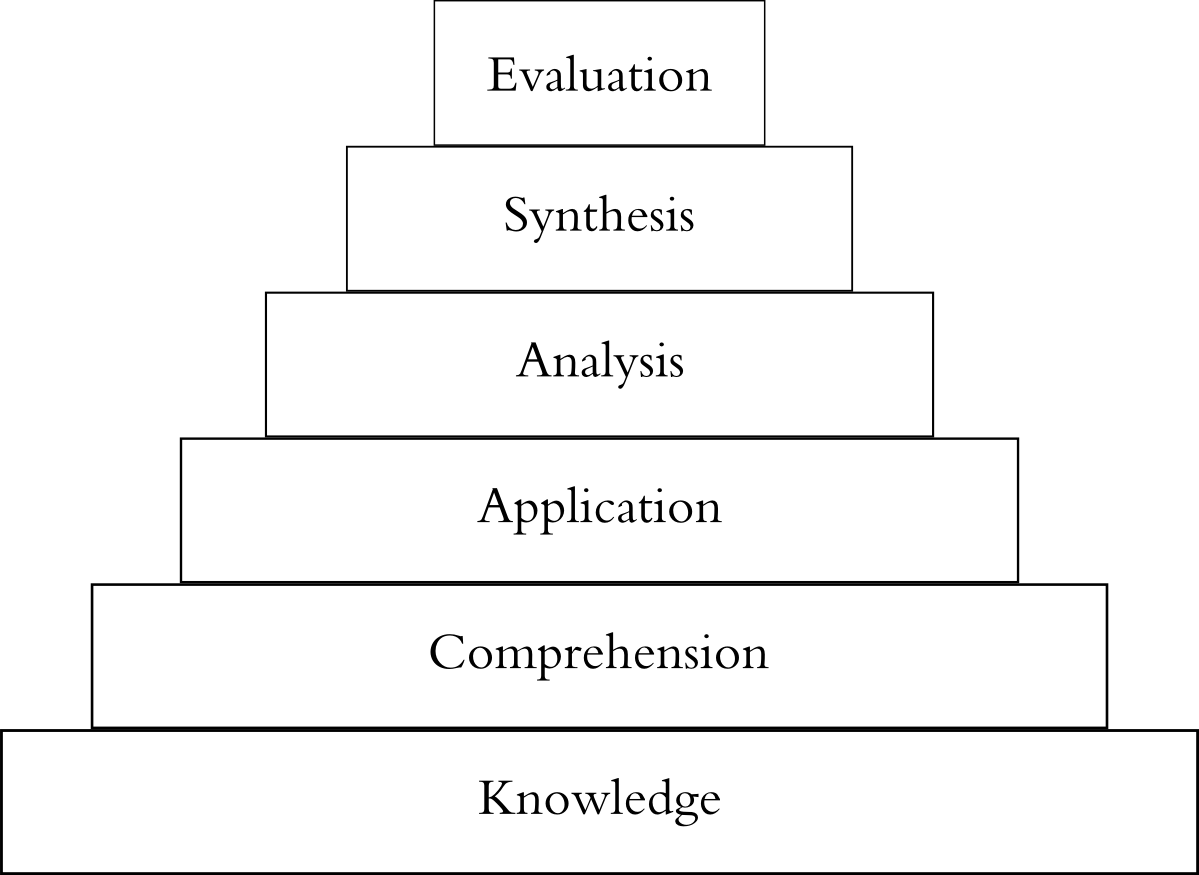
\includegraphics[width=.4\textwidth]{bloom}
\caption{The taxonomy of Bloom \protect\cite{bloom}\label{fig:bloom}}
\end{figure}

36 of the learning objectives fall into the knowledge domain within the taxonomy of Bloom, 15 learning objectives fall into the comprehension domain, 3 learning objectives into the application domain, and 2 objectives into the analysis domain. The reason why most of the learning objectives fall into the knowledge domain is because the topic of quantum mechanics is mainly new to the high school student. Because of this, the student first has to learn a lot of new terms and definitions before he can actually comprehend quantum mechanics, for having knowledge is a prerequisite for an eventual understanding of the concepts. However, the main goal of the instruction is comprehension of the concepts, even if there are only 15 learning objectives within this domain, for comprehension leads to conceptual understanding. Application and Analysis is less relevant, this would be more relevant to principle learning, which would be important for learning the algorithmic aspects of quantum mechanics. Any higher domains cannot be reached, for they require mastery of the application and analysis domain. However, this could be achieved next in the curriculum.

Furthermore, the learning objectives are also categorised by topical domains, which are Applications of Quantum MechanicsPre-knowledge, Elementary Particles, Classical Communication, Observation Dependency, Realism and Ontology, Superposition, Entanglement, Uncertainty Principle of Heisenberg and Teleportation. Each instruction should start with a reason why the student might be interested in learning the subject. This is established by stating the relevance of quantum mechanics by enlisting the different applications of quantum mechanics.

When the student knows why he should learn about quantum mechanics, the instruction continues with what the student already might know, because this activates the brain regions containing this information, making it possible for the student to connect the new knowledge with what he already knows. As already stated in the \emph{Learner Analysis} on page~\pageref{sec:learneranalysis}, the student should already be familiar with the Rutherford-Bohr model of the Atom. This thereupon leads easily into the next domain, namely that of the \emph{Elementary Particles}. Here, the student learns about the particles which demonstrate quantum behaviour.

When learned about the existence of elementary particles, the student can also learn about \emph{Classical Communication}. This needs understanding about elementary particles, for these are the particles which are used to conduct classical communication. Classical communication is relevant to quantum mechanics for two reasons. The first reason is that it connects the mysterious elementary particles to the daily experience. Everyone uses the internet everyday, which uses classical communication. Therefore, the student should already be familiar with the concept. The second reason is that it is a prerequisite for learning about quantum teleportation, which will be explained later on in this section.

It might strike the reader that the famous double-slit experiment is not entailed within the learning objectives. There are two reasons for not including this experiment in the instruction. First of all, the double-slit is already part of the standard curriculum \cite{eindexamen2015}, so there is no need to develop educational material for it. The second and more important reason is that the double-slit experiment can be used to demonstrate the relations between the concepts within quantum mechanics, but to fully comprehend these relations the student should first learn the concepts themselves. The term "wave-particle duality" also does not hold any meaning if the student is still unaware of the probabilistic nature of quantum mechanics. However, this instruction could be followed up by instruction covering the double-slit experiment.

The first concept underlying the double-slit experiment is \emph{Observer Dependency}. This is also the first time the student is confronted by one of the more counterintuitive concepts of quantum mechanics. It teaches the student that quantum mechanics cannot only be explained by pure determinism and causal relations, but that quantum mechanics has a probabilistic nature. The student learns this concept by examining what happens if a property of an elementary particle is observed.

The probabilistic nature of quantum mechanics is further explored with the debate between \emph{Realism and Ontology}. This section starts with the realist interpretation of quantum mechanics, which entails that there must be an explanation for the seemingly random behaviour of elementary particles, it is only not possible to measure with the current level of technology. The ontologist explanation however is that there is no explanation of the random behaviour of elementary particles, and it is the inherent nature of quantum mechanics. With this debate, the student is challenged to evaluate his own believes about the nature of physics. Most likely, he will start at the realistic interpretation, and this is a natural way to teach the student to let him think about the other interpretation.

After this historical and philosophical intermezzo, the student is then introduced to the second concept underlying the double-slit experiment, which is \emph{Superposition}. This concept can only be fully understood when the student is aware of the ontologist interpretation, for it involves comprehension of the fact that quantum mechanics is truly probabilistic. This is because the student has to understand that before measurement, the elementary particle has no true defined state yet, and is in all different states at the same time.

The next concept the student is introduced to is the concept of \emph{Entanglement}, which teaches the student that the behaviour of elementary particles is not entirely random. Although the collapse of two entangled particles is fundamentally random, the two particles are interdependent. This means that the particles can either collapse to the same state on observation in the case of bosons, or that the particles collapse to each others opposite state in the case of fermions. This concept could be used to develop further in the EPR experiment, which was an attempt of realist interpreters to prove that there is an underlying explanation of quantum mechanics, but ultimately led to more evidence for the ontologist interpretation. The EPR experiment makes way for topics like the hypothesis of locality, the hidden variable hypothesis and Bell's inequalities. However, this instruction will limit itself to only explaining the concept of entanglement itself, for the EPR experiment is quite sizeable and fits in an entire separate instruction.

The next topic is the \emph{Uncertainty Principle of Heisenberg}, which stands a bit on its own. It can be used to teach the student about the non-locality of quantum mechanics, because it demonstrates that the specific location or the specific speed of an elementary particle cannot be known exactly, and there is an inherent uncertainty about these two variables. Furthermore, it also has a different realist and ontologist interpretation. To understand the ontologist interpretation, it is important that the student is already taught about superposition. The reason why this topic is included in the instruction is because it is another counterintuitive but central concept within quantum mechanics, and it is regarded as important for teaching by \citeA{henriksen}. The principle is also one of the few topics directly included in the Centraal Eindexamen 2016 \cite{eindexamen2016} within this instruction. Finally, it also ties in with the next domain.

This last domain is \emph{Teleportation}, which teaches the student about the inner workings of entanglement in the real world. This topic will first explain what it is not, but is easily confused with, namely the teleportation used in science-fiction. To argue that this is actually not possible, the student has to use the uncertainty principle of Heisenberg. This is also the main reason that it is included, all the topics taught before have to be used in the Teleportation experiment, it can therefore  serve as a conclusion of the instruction by letting the student go through all the different domains one more time.

\subsection{Test specifications}

Every learning objective has to contain a description of the terminal behaviour or actions that will demonstrate learning, a description of the conditions of demonstration of that action and a description of the standard or criterion \cite{smithragan}. The description of the terminal behaviour is already specified in the \emph{Learning Objectives} appendix on page~\pageref{app:learningobjectives}. If a condition is present for the execution of the learning objective, this is already specified as well, most of the time using the word "given". However, the standards or criteria for measuring specifying how the learning objective has to be achieved by the student are not yet included in the table.

Thinking about the criteria or standards on beforehand can be very useful for the designer, for he then also has an idea for how specific the instruction text should be written. Therefore, a list with the standards given a certain learning objective has also been included, in the \emph{Learning Objectives and Standards} appendix on page~\pageref{app:objectivestandards}. The objectives are indicated by numbers, and the standards by letters. The standards are formulated as the behaviour the student should display upon measurement of the learning objective. Some of the learning objectives are formulated in such a way that further specification by standards is not necessary, for example learning objective~\ref{itm:molecules}: "The student can state that everything we observe exists out of molecules".

\section{Evaluation}

To ensure that the instruction would not contain errors on the subject of quantum mechanics, an expert was consulted to look at the learning objectives and criteria. The expert consulted is a part-time PhD student which researched the implementation of quantum mechanics in the curriculum of Dutch secondary education, and a part-time first grade physics teacher. The same expert was also consulted during the Needs Assessment (see page~\pageref{sssec:problem}). For this evaluation, a focus group evaluation was conducted \cite{evamatchboard}. With the walkthrough, the design proposal was checked on factual errors, using an interview with the expert. The result of the walkthrough would be an evaluation of the relevancy and the consistency of the product (see the \emph{Evaluation Matchboard} appendix on page~\pageref{app:evamatchboard}), which entailed going through all the learning objectives and standards. Although she gave  feedback on the specific formulation of some of the learning objectives or criteria, she did not find any factual errors. She did give some feedback on which learning objectives might not be considered to be pre-knowledge, such as learning objective~\ref{itm:planckconstant}: "The student can state the value of the reduced Planck Constant".

%%% DESIGN

\chapter{Design}
\thispagestyle{fancy}

The second phase of the Generic Model is the Design phase \cite{genericmodel} (see figure~\ref{fig:genericmodel} on page~\pageref{fig:genericmodel}). In this phase, the results from the Analysis phase are translated into design principles and an outline of the instruction that can be used directly for the development of the instruction. This chapter will start out with the relevant conclusions which are drawn from the analysis phase in order to summarise the results and translate them to the context of the product, the instruction. After the summary, an active choice still has to be made about the medium to use for delivering the instruction. This will be done in the next section according to the results relevant to the choice of the medium. The remaining conclusions will then be used to formulate design principles, which facilitate the concrete use of the results from the analysis. Furthermore, design principles can be used after the development for a screening evaluation \cite{evamatchboard} (see the Evaluation Matchboard appendix on page~\pageref{app:evamatchboard}). Finally, the different learning objectives formulated during the task analysis have to be ordered into an outline of the instruction, so the designer can directly translate them into text or other means of instruction.

\section{Conclusions from the Analysis}

There is a wide variety of topics available for quantum mechanics education. It is advisable to start any instruction with the Rutherford-Bohr model of the Atom and its relation to elementary particles, for this is the scale on which quantum mechanics take place. A next step could be introducing the different phenomena which happen on a quantum scale, such as superposition, observer dependency and entanglement. One way to introduce superposition and observer dependency is by using the double-slit experiment. This also teaches about the wave-particle duality of elementary particles. Furthermore, the students could be taught the differences between classical mechanics and quantum mechanics, which are determinism and probabilism, locality and non-locality, and continuous and discrete distances. One way to highlight the strangeness of quantum mechanics is by using the debate between realism and ontology, this emphasises that quantum mechanics are different than a student might think at first. There are also famous thought experiments, for example Schrödinger's cat, which could be used to create different mental models with the students. Finally, there are some mathematical approaches to quantum mechanics, however there is a consensus within educators that a conceptual approach is more effective.

Not a lot of studies write why quantum mechanics should be taught on secondary education. There is however no study which claimed it should not be taught. Reasons why it should be taught are that educated citizens should be acquainted with quantum mechanics and that it is regarded fundamental.

Quantum mechanics is regarded to be a difficult topic, because it is counter intuitive, it contradicts daily experienced locality and determinism, it is regarded to be abstract, it is difficult to visualise and it is mathematically challenging.

Misconceptions about quantum mechanics can arise out of the nature of quantum theory, but also from textbooks and previous instruction. It is important that the information handed to the students are not simplified, because this can lead to misconceptions. Problems also often originate from outdated deterministic or realist models. The students therefore have to be confronted with the fact that their own models cannot be applied in the context of quantum mechanics. Students also find it difficult to recognise the scale in which quantum mechanics take place. Hence, the students should be informed that quantum mechanics take place on the scale of elementary particles. Knowledge of students often consists out of memorised facts, and when confronted with new or different information, new facts are memorised instead of creating right models. This results in fragmented incorrect but self-consistent models. Because of this, the instruction should provide the student with a coherent description of quantum mechanics.

The literature prescribes different strategies for teaching quantum mechanics, namely recommendations for content, aspects of the medium to use, meta-cognitive aspects and a framework. Content related strategies entail embedding the instruction in real-world contexts, letting the student appreciate the relevance of quantum mechanics, introducing microscopic processes as an integral part of electricity and magnetism, using the language of physics, and using an conceptual approach instead of a mathematical approach. The medium used should be interactive, it should visualise the concepts, it should make use of different modes of representation, and it should make use of computation. It should be noted however that one should be careful with visualisation, for this can easily lead to misconceptions. The use of simulations are suggested. Furthermore, critical thinking skills, active learning, feedback and collaborative learning could contribute to students building the correct mental models of how quantum mechanics work. Finally, thought experiments are regarded to be very effective for learning quantum mechanics, this entails questions and general assumptions, a description of the features of the system, performance of the thought experiment itself, extraction of the results and drawing conclusions.

In secondary education, instructions often emphasise learning and practising algorithmic skills. This however clashes with the recommendations from the literature, which advocates an emphasis on conceptual understanding. It is also found that students show higher interest in conceptual aspects than the algorithmic aspects. Conceptual approaches engage students and probes the student to ask fundamental questions. Because of the focus on algorithmic aspects, students currently often do not learn what is intended by the developer of the instruction, improved student learning might be possible by shifting the focus to conceptual understanding. This is why the learning objectives are all targeted towards a better conceptual understanding of the student, without having to rely on complex mathematics or experiments. The different domains which will be taught are Applications of Quantum Mechanics, Pre-knowledge, Elementary Particles, Classical Communication, Observation Dependency, Realism and Ontology, Superposition, Entanglement, and the Uncertainty Principle of Heisenberg. These Domains will then be combined within the experiment of Quantum Teleportation.

\section{The Medium}

\subsection{Requirements for the Medium}

The analysis phase provides a couple of recommendations or requirements for the medium used to deliver the instruction:

\begin{itemize}
\item The medium should allow interaction;
\item The medium should be able to visualise the content;
\item The medium should be able to use different modes of representation;
\item The medium should take away the mathematical difficulty, for example by using computation.
\end{itemize}

As already stated within the Analysis chapter, these requirements cannot be reached by relying on traditional means of instruction such as text books, pictures and lectures from a teacher. It is not possible for a student to interact with the contents of a book or with pictures, and lectures from a teacher often entail the teacher standing in front of the class and telling the students about quantum mechanics in a supplantive way. Of course it would be possible for a student to ask questions, but more room for interaction is needed to be even more successful, and the teacher has not enough time to facilitate interactive learning to every student in a differentiated way.

One of the suggestions from the studied literature entailed using simulations, because these could provide all of the requirements. However, simulations often are related to certain experiments, for example by simulating the double-slit experiment and providing the student with data such as visuals or numerals. This is in contrast with the requirements from the task analysis, which specify that rather than teaching by means of experiments, the instruction should first teach about the concepts themselves in a more direct way.

Another way of teaching quantum mechanics via electronic media would be to deliver the instruction by using game-based learning. game-based learning refers to the use of games for educational purposes. Relatively speaking, only little research has been carried out to investigate game-based learning, but recent reviews revealed a potential of games being an effective tool for instruction, "even more effective than conventional instruction" \cite[p.~1]{wouters}. In order for game-based learning to take place, the game has to supersede sole entertainment purposes by having an educational value, so that the player learns something about the real world by playing the game. Examples of these games are historical games like Assassin's Creed, Age of Empires or Valiant Hearts, in which the player is exposed to certain historical events or figures, or puzzle games like Portal, in which the player develops an understanding about physics. However. these games are often only intended for entertainment purposes and are only tangentially fit for educational purposes. Most research within game-based learning is conducted on games which are specifically designed to have an educational value. These games often contain explicit formulated learning goals which can be tested by pre- and post-testing. They are designed with the primary goal of education rather than entertainment, and are therefore a subset of Serious Games. This term refers to the set of games designed for a primary goal other than pure entertainment. This goal can be teaching, but also raising awareness about a certain topic or persuading the player to believe something.

One disadvantage for using game-based learning is that it takes a lot of time to develop games in general, and there is no game available on the market which can be directly used for teaching the learning objectives specified in the Task Analysis. However, there already exists an easy to use engine which can be used to teach quantum mechanics on a conceptual level. This engine is qCraft, developed as a modification for the game Minecraft.

\subsection{Minecraft}

Minecraft is a game initiated by Marcus Persson (also known as Notch), further developed by Mojang AB, and now property of Microsoft. It is available for Windows, OS X, Linux, Java platform, Java applet, Android, iOS, Windows Phone, Amazon Fire TV, Xbox 360, Xbox One, Rasberry Pi, Playstation 3, Playstation 4, and the Playstation Vita. There are differences between the versions, and the main version is being developed for the PC only. It is the third-best sold game of all time, and the best sold game for PC with 70 million sold copies at the time of writing.

The game is a first person sandbox survival game, available for playing both in single-player and multiplayer. In the game, the player walks around in a procedurally generated world fully made out of blocks which are one cubic meter in size (see figure~\ref{fig:screenshot}). The player can control his avatar similar to other first person games, by using the WASD keys for moving and using the mouse for looking around. The unique feature of the game is that the player can place and remove blocks for himself. Each block also has a specific block-type, which gives it a certain appearance and sometimes also a special physical attribute. For example, blocks with the sand block-type always fall down unless being on top of another block. Some blocks also emit a signal, which can be used to trigger certain commands or for example open a door to a room.

\begin{figure}[h]
\centering
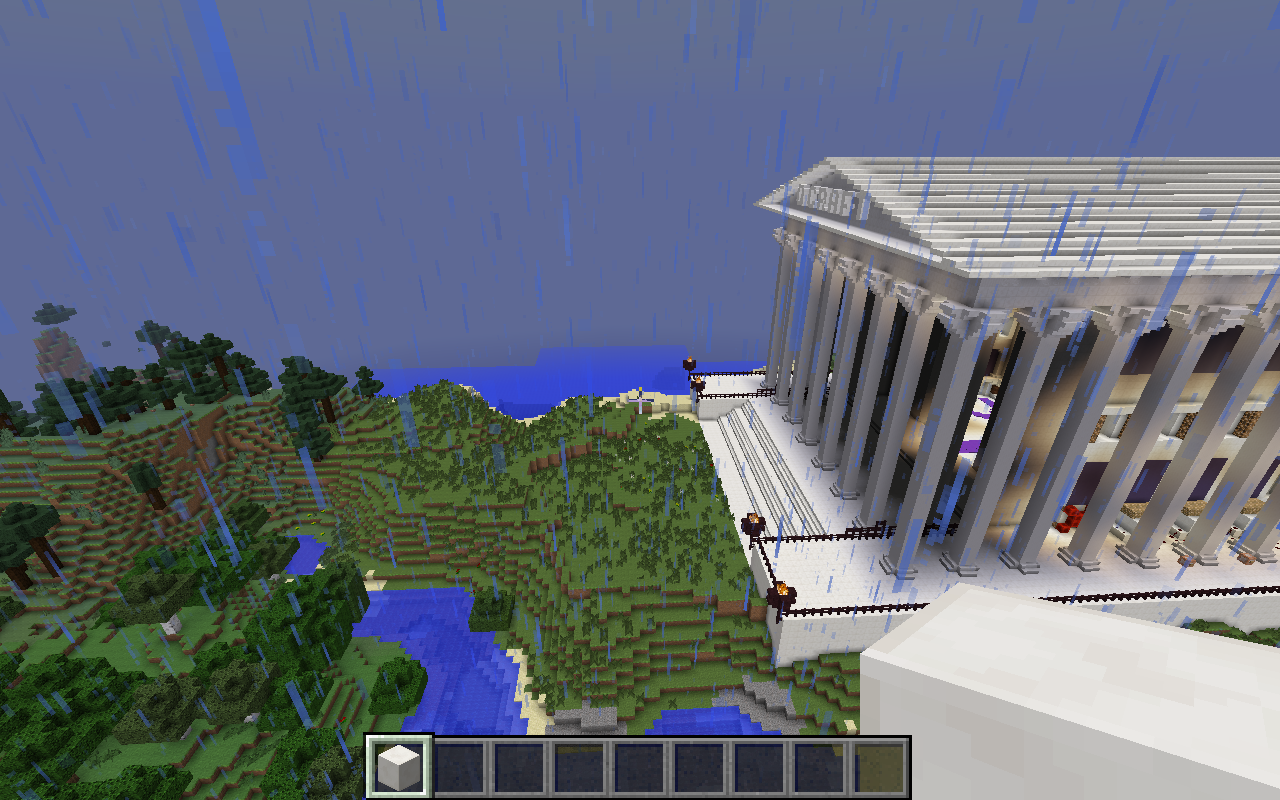
\includegraphics[width=\textwidth]{screenshot}
\caption{A screenshot within the game Minceraft, where a player created structure is placed within the procedurally generated terrain.\label{fig:screenshot}}
\end{figure}

Minecraft is an easy to use engine for delivering instructions as well. It has support for signs with text and pictures which can be placed in the world, books the player can open and read, and commands which can be used to move the player to certain areas in the world or giving the player certain items. There is even a special version of Minecraft for use in classrooms, which is called MinecraftEdu (\url{minecraftedu.com}), and it is used by teachers around the world.

\subsection{qCraft}

In order to use Minecraft to students, a certain modification of the game has to be installed. This modification is also available for MinecraftEdu, which makes it easier to use for teachers. The mod introduces special types of blocks into the game, which are Observer Dependent Blocks and Quantum Blocks. The Quantum Blocks behave in a way similar to elementary particles, which is that every time a Quantum Block is observed, it first is in a green "in-between state" and then takes on one of two block-types at random. An observation takes place every time the player looks at it. For example, if a player looks at a Quantum Block, it can collapse 50\% of the time to a gold block-type and 50\% of the time to a diamond block-type. The green colour the block takes on before collapsing to either of the two block-types represents the fact that the block is in superposition before measurement.

An Observer Dependent Block has one difference with the Quantum Block, which is that its block-type does not collapse at random, but that the collapse is determined by the angle the block is observed from. This block is added to the game in order to learn the student observer dependency, without also having to explain the random collapse. 

Quantum Blocks can also be entangled with each other. This means that every time one of the entangled blocks is observed, all Quantum Blocks their block-type collapse to the same value. Only the boson type of entanglement is implemented yet.

Furthermore, the modification adds a couple of tools to interact with the blocks. It adds two types of goggles, which are the Quantum Goggles and the Anti-Observation Goggles. The Quantum Goggles highlight all of the special blocks by giving it a fluorescent green colour, so the player can easily identify all of the qCraft blocks present around him. The Anti-Observation Goggles prevent the player from generating observations to the qCraft blocks. Another tool provided by qCraft is the Automatic Observer, which can be activated to generate an observation to the qCraft block attached to the Automatic Observer.

\subsection{Possibilities of using qCraft for teaching quantum mechanics}

First of all, qCraft meets all the requirements earlier specified based on recommendations by the studied literature. It is interactive, because the student can move around in the world instead of being a passive observer. This allows for walking around the qCraft block, observing them in different ways, trying to find the patterns, and even trigger mechanisms based on the collapse of the block type of the qCraft block. Furthermore, the mechanics introduced by qCraft make quantum mechanics visible. The player can see what observer dependency means for a Quantum Block, and how boson type entanglement works between multiple Quantum Blocks. One of the advantages of using Quantum Blocks is that they already demonstrate the correct behaviour, so there is no need to rely on thought experiments such as Schrödinger's Cat. The student can observe the behaviour directly, and can therefore experiment with it without needing an external analogy. Minecraft also allows for different modes of representation. Next to the qCraft blocks, it is also possible to hang pictures in the world, to place text on signs, and to add books into the world. This allows for explaining the players the specific behaviour of the blocks and to transfer this to real quantum mechanics by comparing it to the behaviour of elementary particles. Additionally, the only mathematical comprehension the player needs in order to understand the behaviour of the blocks is that the block types collapse to a random state, without having to comprehend difficult probability functions which require mathematical skills which students of secondary education do not possess.

Finally, all of the learning objectives can be achieved using only qCraft, without having to rely on more external sources of delivery. One disadvantages of using qCraft is that it is not possible to visualise the double-slit experiment for example. However, it was already stated in the Analysis phase that this experiment would occur only after a conceptual understanding was achieved with the student, and that it could be introduced later on in the curriculum. The debate between realism and ontology can be described within a book. The uncertainty principle of Heisenberg cannot be emulated within qCraft. However, it is possible to display the different variables within the formula on images situated in the world. This way the student can learn the formula by means of discovery learning. The experiment of teleportation is visualisable in qCraft, for the only concepts needed are random collapse and entanglement.

Another advantage of using qCraft is its accessibility. A lot of people already play Minecraft, and this could be an attractive entrance into the world of quantum mechanics. There are also a lot of gamers who have not yet played Minecraft, but are still quite familiar with the controls because they have played other first person games. However, there will also be students who are not familiar with first person games, so a tutorial teaching the controls of Minecraft will still be needed at the beginning of the instruction.

\section{Design Principles}

Most of the recommendations from the studied literature are already covered by the choice of learning objectives and the choice for qCraft. Other recommendations are not directly relevant to the design of the instruction, for they are recommendations relevant to the implementation of the instruction, which will not be done within this project. However, there are still a couple of recommendations which are still relevant for consideration during the development phase. Therefore, these recommendations have been translated into a list of design principle in the list below.

\begin{enumerate}
\item \label{itm:simple}The information handed to the student are not allowed to be simplified, for this can lead to misconceptions
\item \label{itm:language} The language of physics has to be used to teach students the concepts within quantum mechanics
\item \label{itm:links}The different concepts have to be connected with each other
\item \label{itm:realworld}Each concept should be transferred to the real-world context of the behaviour of elementary particles
\item \label{itm:maths}The instruction has to be mathematically accessible towards the student and should not require mathematical skills beyond those of physics student within upper secondary education
\item \label{itm:models}Students have to be triggered to reconsider their realist or deterministic models of physics in the context of quantum mechanics
\item \label{itm:critic}The critical thinking skills of the student have to be activated
\item \label{itm:active}The student has to be triggered into having an active learning style
\item \label{itm:results}The student has to be asked to extract results from his observations
\item \label{itm:conclusions}The student has to be asked to draw conclusions from the extraction of the results
\item \label{itm:feedback}The student has to get feedback on the conclusions he has drawn
\end{enumerate}

Someone might notice that the design principles are quite broadly defined, whereas normal design principles are formulated in a more concrete way. However, due to the nature of this project, the only source for these design principles are the recommendations by the literature. As such, the concreteness of the design principles are dependent on how concrete the recommendations are defined within the articles. Still, these design principles can be used as general guidelines for developing the instruction.

Design principle~\ref{itm:simple} is especially relevant when visualising any concepts for the reader. This might be especially relevant when depicting the Rutherford-Bohr model of the Atom, for this easily leads to a conception of an electron orbiting around the nucleus, whereas the electron is just somewhere in the shell and not at a specific location in orbit with a specific speed. A way around this is by using figure~\ref{fig:bohrmodel} on page~\pageref{fig:bohrmodel}, for this displays only the nucleus and the shell without an electron particle.

To provide the students with handles to internalise the concepts, the terminology of quantum physics will be used as specified in principle~\ref{itm:language}. The aim of principle~\ref{itm:links} is preventing fragmented incorrect but self-consistent models. By connecting and combining the different concepts, the student is able to build one holistic model of quantum mechanics, instead of developing disconnected models about different experiments. A way to connect the concepts is by repeating the concepts, actively explaining  the relations between the concepts and finally combining all of the concepts in the teleportation experiment. Another way to connect the different concepts is by relating them all to the behaviour of elementary particles, which is stated in principle~\ref{itm:realworld}. This also places the concepts in a context which is familiar to the student, for he already learned about electrons and photons earlier during physics lessons.

The design principle~\ref{itm:maths} related to the mathematical level is probably already covered by the choice of learning objectives and the choice of medium of delivery. However, it still remains an important requirement for the instruction because most current instructions make the mistake of underestimating the mathematics, and it is therefore included.

Design principles~\ref{itm:models},~\ref{itm:critic}, and~\ref{itm:active} are important to help the student realise the counterintuitive aspects of quantum mechanics. This can be achieved by asking the student questions about the material and about his own beliefs. Principles~\ref{itm:results} and~\ref{itm:conclusions} then trigger the students to actively build new mental models about physics. Finally, design principle~\ref{itm:feedback} provides the students with feedback on their newly built mental models, so they can adjust them towards a more correct model.

\section{Outline of the Instruction}

The last step of the design phase is to structure the learning objectives in such a way that the instruction can be written.

\subsection{Learning Events of Instruction}

\subsection{Types of Learning}

\subsection{Supplantive and Generative Instruction}

%%% DEVELOPMENT

\chapter{Development}
\thispagestyle{fancy}

%%% FORMATIVE EVALUATION

\chapter{Formative Evaluation}
\thispagestyle{fancy}

\bibliographystyle{apacite}
\bibliography{references}

\chapter{Appendices}

\appendix

\section{Learning objectives}
\label{app:learningobjectives}


\begin{table}[htbp]
\small
\begin{center}
\begin{tabular}{|c|p{5cm}|p{1.5cm}|c|p{3cm}|}
\hline
\textbf{\#} & \textbf{Name} & \textbf{\footnotesize Prerequisite} & \textbf{Taxonomy of bloom} & \textbf{Domain} \\ \hline
1 & The student can list the different applications of quantum mechanics &  & Knowledge & Applications of Quantum Mechanics \\ \hline
2 & The student can state that everything we observe exists out of molecules &  & Knowledge & Pre-knowledge \\ \hline
3 & The student can state that molecules exist out of atoms & 2 & Knowledge & Pre-knowledge \\ \hline
4 & The student can state that atoms exist out of protons, neutrons and electrons & 3 & Knowledge & Pre-knowledge \\ \hline
5 & The student can state what a photon is &  & Knowledge & Pre-knowledge \\ \hline
6 & The student can state the speed of light & 5 & Knowledge & Probably pre-knowledge \\ \hline
7 & The student can state the value of the diameter of an atom & 3 & Knowledge & Might be pre-knowledge \\ \hline
8 & The student can state the value of the Planck Constant &  & Knowledge & Might be pre-knowledge \\ \hline
9 & The student can state that protons exist out of 2 up-quarks and 1 down-quark & 4 & Knowledge & Might be pre-knowledge \\ \hline
10 & The student can state that neutrons exist out of 1 up-quark and 2 down-quarks & 4 & Knowledge & Might be pre-knowledge \\ \hline
11 & The student can state that protons and neutrons are about as heavy, and that electrons have an insignificant weight compared to the other two & 4 & Knowledge & Pre-knowledge \\ \hline
12 & The student can state that opposite charged particles attract each other & 4 & Knowledge & Pre-knowledge \\ \hline
13 & The student can state that protons are positively charged & 4 & Knowledge & Pre-knowledge \\ \hline
14 & The student can state that electrons are negatively charged & 4 & Knowledge & Pre-knowledge \\ \hline
\end{tabular}
\end{center}
\label{completeoutline}
\end{table}
\begin{table}[htbp]
\small
\begin{center}
\begin{tabular}{|c|p{5cm}|p{1.5cm}|c|p{3cm}|}
\hline
15 & The student can state that neutrons do not have any charge & 4 & Knowledge & Pre-knowledge \\ \hline
16 & The student can state that photons, electrons and quarks are elementary particles & 9, 10 & Knowledge & Elementary Particles \\ \hline
17 & The student can state the definition of an elementary particle & 16 & Knowledge & Elementary Particles \\ \hline
18 & The student can explain what an elementary particle is & 17 & Comprehension & Elementary Particles \\ \hline
19 & The student can state that classical Communication happens by sending particles through a channel & 18 & Knowledge & Classical Communication \\ \hline
20 & The student can state that no particle can travel faster than light & 6 & Knowledge & Classical Communication \\ \hline
21 & The student can explain why messages through a classical communication channel cannot travel faster than the speed of light & 19, 20 & Comprehension & Classical Communication \\ \hline
22 & The student can calculate the time needed to send a message from location A to location B using classical communication given the distance between A and B & 21 & Application & Classical Communication \\ \hline
23 & The student can state certain properties of elementary particles & 11, 12, 13, 14, 15 & Knowledge & Observation Dependency \\ \hline
24 & The student can state that a property of an elementary particle collapses to a certain value on observation & 23 & Knowledge & Observation Dependency \\ \hline
25 & The student can state that the collapse of a property of an elementary particle to a certain value is random & 24 & Knowledge & Observation Dependency \\ \hline
26 & The student can explain what happens to the property of an individual elementary particle if it is observed & 25 & Comprehension & Observation Dependency \\ \hline
27 & The student can list the two different interpretations of quantum mechanics &  & Knowledge & Realism and Ontology \\ \hline
28 & The student can state the realist interpretation of the collapse of a property & 26, 27 & Knowledge & Realism and Ontology \\ \hline
29 & The student can state the ontologist interpretation of the collapse of a property & 26, 27 & Knowledge & Realism and Ontology \\ \hline
30 & The student can explain the realist interpretation of quantum mechanics & 28 & Comprehension & Realism and Ontology \\ \hline
31 & The student can explain the ontologist interpretation of quantum mechanics & 29 & Comprehension & Realism and Ontology \\ \hline
\end{tabular}
\end{center}
\end{table}
\begin{table}[htbp]
\small
\begin{center}
\begin{tabular}{|c|p{5cm}|p{1.5cm}|c|p{3cm}|}
\hline
32 & The student can differentiate between a realist interpretation and an ontological interpretation of quantum mechanics, given a statement of either a realist interpretation or an ontologist interpretation & 30, 31 & Comprehension & Realism and Ontology \\ \hline
33 & The student can state that before observing a property of an elementary particle, it is in a state of superposition & 31 & Knowledge & Superposition \\ \hline
34 & The student can state the definition of superposition & 33 & Knowledge & Superposition \\ \hline
35 & The student can explain in what state the property of an elementary particle is before observing this property & 34 & Comprehension & Superposition \\ \hline
36 & The student can state the definition of entanglement & 26 & Knowledge & Entanglement \\ \hline
37 & The student can state that entanglement occurs between two elementary particles & 27 & Knowledge & Entanglement \\ \hline
38 & The student can state that entanglement can take place no matter the distance between the two particles & 37 & Knowledge & Entanglement \\ \hline
39 & The student can state that entanglement can take place no matter when each particle is observed & 37 & Knowledge & Entanglement \\ \hline
40 & The student can list the two different types of entanglement & 28 & Knowledge & Entanglement \\ \hline
41 & The student can state that the properties of two boson entangled particles always collapse to the same state & 29 & Knowledge & Entanglement \\ \hline
42 & The student can state that the properties of two fermion entangled particles always collapse to each others opposite state & 29 & Knowledge & Entanglement \\ \hline
43 & The student can explain what happens to the properties of two entangled particles on observation & 41, 42 & Comprehension & Entanglement \\ \hline
44 & The student can use entanglement to predict which state the property of a particle will collapse to, given the state of the property of an entanglement particle and the type of entanglement between the two particles & 43 & Application & Entanglement \\ \hline
45 & The student can deduce the type of entanglement given the states of a common property between two entanglement particles & 43 & Analysis & Entanglement \\ \hline
46 & The student can state the uncertainty principle of Heisenberg & 8, 17 & Knowledge & Uncertainty Principle of Heisenberg \\ \hline
\end{tabular}
\end{center}
\end{table}
\begin{table}[htbp]
\small
\begin{center}
\begin{tabular}{|c|p{5cm}|p{1.5cm}|c|p{3cm}|}
\hline
47 & The student can explain the meaning of each variable in the uncertainty principle of Heisenberg & 46 & Comprehension & Uncertainty Principle of Heisenberg \\ \hline
48 & The student can explain why the exact location or momentum cannot be known according to the uncertainty principle of Heisenberg & 47 & Comprehension & Uncertainty Principle of Heisenberg \\ \hline
49 & The student can explain why the position has to be lesser known if the momentum is better known and vice versa according to the uncertainty principle of Heisenberg & 47 & Comprehension & Uncertainty Principle of Heisenberg \\ \hline
50 & The student can explain why the uncertainty principle of Heisenberg is only significant when dealing with very small objects & 7, 47 & Comprehension & Uncertainty Principle of Heisenberg \\ \hline
51 & The student can differentiate between the measurement of the location of a planet and the measurement of the location of an electron & 50 & Comprehension & Uncertainty Principle of Heisenberg \\ \hline
52 & The student can list the steps of teleportation in science-fiction movies &  & Knowledge & Teleportation \\ \hline
53 & The student can explain why science-fiction teleportation is not possible & 48 & Comprehension & Teleportation \\ \hline
54 & The student can list the steps of quantum teleportation & 43 & Knowledge & Teleportation \\ \hline
55 & The student can explain what happens when conducting quantum teleportation & 54 & Comprehension & Teleportation \\ \hline
56 & The student can apply the correct step from the quantum teleportation experiment, given a certain situation & 55, 44, 45 & Application & Teleportation \\ \hline
57 & The student can deduce why quantum teleportation cannot be used to communicate instantly with someone on a different location & 55 & Analysis & Teleportation \\ \hline
\end{tabular}
\end{center}
\caption{A complete outline of the learning objectives used for the instruction. With each learning objective, the name, the direct prerequisites, the category within the taxonomy of Bloom and the domain is provided.}
\label{completeoutline}
\end{table}

\newpage

\section{Learning Objectives and Standards}
\label{app:objectivestandards}

\begin{enumerate}
\item The student can list the different applications of quantum mechanics
\begin{enumerate}
\item The student enlists the transistor as an application of quantum mechanics
\item The student enlists the laser as an application of quantum mechanics
\item The student enlists quantum computing as a possible future application of quantum mechanics
\end{enumerate}
\item \label{itm:molecules} The student can state that everything we observe exists out of molecules
\item The student can state that molecules exist out of atoms
\item The student can state that atoms exist out of protons, neutrons and electrons
\item The student can state what a photon is
\begin{enumerate}
\item The student states that a photon is a light particle
\end{enumerate}
\item The student can state the speed of light
\begin{enumerate}
\item The student states that the speed of light is about $3.0 \cdot 10 ^ 8$ m/s
\end{enumerate}
\item The student can state the value of the diameter of an atom
\begin{enumerate}
\item The student states that the value of the diameter of an atom is 0.1 to 0.5 nm
\end{enumerate}
\item \label{itm:planckconstant}The student can state the value of the reduced Planck Constant
\begin{enumerate}
\item The student states that the Planck Constant is $1.0 \cdot 10 ^ {-34}$ Js 
\end{enumerate}
\item The student can state that protons exist out of 2 up-quarks and 1 down-quark
\item The student can state that neutrons exist out of 1 up-quark and 2 down-quarks
\item The student can state that protons and neutrons are about as heavy, and that electrons have an insignificant weight compared to the other two
\item The student can state that opposite charged particles attract each other
\item The student can state that protons are positively charged
\item The student can state that electrons are negatively charged
\item The student can state that neutrons do not have any charge
\item The student can state that photons, electrons and quarks are elementary particles
\item The student can state the definition of an elementary particle
\begin{enumerate}
\item The student states that it is a particle of which its substructure is not known
\end{enumerate}
\item The student can explain what an elementary particle is
\begin{enumerate}
\item The student uses the definition of an elementary particle to explain what it is
\item The student states that some scientists believe they have no substructure
\end{enumerate}
\item The student can state that classical communication happens by sending particles through a channel
\item The student can state that no particle can travel faster than light
\item The student can explain why messages through a classical communication channel cannot travel faster than the speed of light
\begin{enumerate}
\item The student states that particles are used in certain pattern for classical communication
\item The student states that in order to communicate from one location to another, the particles have to travel between the locations through a communication channel
\item The student states that no particles can travel faster than light
\end{enumerate}
\item The student can calculate the time needed to send a message from location A to location B using classical communication given the distance between A and B
\begin{enumerate}
\item The student divides the distance by the speed of light to derive the time needed
\end{enumerate}
\item The student can state certain properties of elementary particles
\begin{enumerate}
\item The student states charge as a property of an elementary particle
\item The student states polarisation as a property of photons
\end{enumerate}
\item The student can state that a property of an elementary particle collapses to a certain value on observation
\item The student can state that the collapse of a property of an elementary particle to a certain value is random
\item The student can explain what happens to the property of an individual elementary particle if it is observed
\begin{enumerate}
\item The student states that a property of an individual elementary particle will collapse to a random state upon observation
\end{enumerate}
\item The student can list the two different interpretations of quantum mechanics
\begin{enumerate}
\item The student enlists realism as an interpretation of quantum mechanics
\item The student enlists ontology as an interpretation of quantum mechanics
\end{enumerate}
\item The student can state the realist interpretation of the collapse of a property
\begin{enumerate}
\item The student states that the realist interpretation of the collapse of a property has an underlying explanation or mechanic which we do not have the technology available for to measure
\end{enumerate}
\item The student can state the ontologist interpretation of the collapse of a property
\begin{enumerate}
\item The student states that the ontologist interpretation of the collapse of a property has no underlying explanation or mechanic but is inherently random
\end{enumerate}
\item The student can explain the realist interpretation of quantum mechanics
\begin{enumerate}
\item The student states that the realist interpretation of quantum mechanics is that every physical theory is grounded in reality
\item The student states that realists believe that every theory can be explained by classical mechanics
\item The student states that realists believe that even the seemingly random phenomena occurring within quantum mechanics can eventually be explained by the rules of classical mechanics
\end{enumerate}
\item The student can explain the ontologist interpretation of quantum mechanics
\begin{enumerate}
\item The student states that the ontologist interpretation of quantum mechanics is that there is no underlying explanation of quantum mechanics
\item The student states that the ontologist interpretation of quantum mechanics is that quantum mechanics is real and happens on its own
\end{enumerate}
\item The student can differentiate between a realist interpretation and an ontological interpretation of quantum mechanics, given a statement of either a realist interpretation or an ontologist interpretation
\item The student can state that before observing a property of an elementary particle, it is in a state of superposition
\item The student can state the definition of superposition
\begin{enumerate}
\item The student states that if a property is in superposition, its state is in all states at the same time
\end{enumerate}
\item The student can explain in what state the property of an elementary particle is before observing this property
\begin{enumerate}
\item The student states that the property is in all states at the same time and collapses to a specific state upon observation
\end{enumerate}
\item The student can state the definition of entanglement
\begin{enumerate}
\item The student states that entanglement entails an interdependence witihin the collapse of two elementary particles
\end{enumerate}
\item The student can state that entanglement occurs between two elementary particles
\item The student can state that entanglement can take place no matter the distance between the two particles
\item The student can state that entanglement can take place no matter when each particle is observed
\item The student can list the two different types of entanglement
\begin{enumerate}
\item The student enlists boson type entanglement
\item The student enlists fermion type entanglement
\end{enumerate}
\item The student can state that the properties of two boson entangled particles always collapse to the same state
\item The student can state that the properties of two fermion entangled particles always collapse to each others opposite state
\item The student can explain what happens to the properties of two entangled particles on observation
\begin{enumerate}
\item The student state that dependent on the type of entanglement, the property of the particles either collapse to the same state or each others opposite state
\item The student states that if the particles are boson type entangled, the properties will always collapse to the same state upon observation
\item The student states that if the particles are fermion type entangled, the properties will always collapse to each others opposite state upon observation
\end{enumerate}
\item The student can use entanglement to predict which state the property of a particle will collapse to, given the state of the property of an entanglement particle and the type of entanglement between the two particles
\begin{enumerate}
\item If the particles are bosons, the student argues that the state to which the property will collapse will be the same as the state of the property of the entangled particle
\item If the particles are fermions, the student argues that the state to which the property will collapse will be the opposite of the state of the property of the entangled particle
\end{enumerate}
\item The student can deduce the type of entanglement given the states of a common property between two entanglement particles
\begin{enumerate}
\item The student argues that if the states of the common property are the same, the two particles must be bosons
\item The student argues that if the states of the common property are the opposite, the two particles must be fermions
\end{enumerate}
\item The student can state the uncertainty principle of Heisenberg
\begin{enumerate}
\item The student states that the uncertainty principle of Heisenberg can be expressed as $\sigma x  \cdot\sigma p \geq \frac{\hbar}{2}$
\end{enumerate}
\item The student can explain the meaning of each variable in the uncertainty principle of Heisenberg
\begin{enumerate}
\item The student states that the $\sigma$ symbol is an expression of uncertainty
\item The student states that the $x$ refers to the location of the particle
\item The student states that the $p$ refers to the momentum of the particle
\item The student states that the momentum is an expression of the speed of a particle
\item The student states that the $\geq$ symbol expresses "greater or equal than"
\item The student states that the $\hbar$ symbol refers to the reduced Planck constant
\item The student summarises this as that the product of uncertainty in location and uncertainty in momentum has to be greater or equal than the reduced Planck constant divided by 2
\end{enumerate}
\item The student can explain why the exact location or momentum cannot be known according to the uncertainty principle of Heisenberg
\begin{enumerate}
\item The student argues that if either $\sigma x$ or $\sigma p$ is 0, $\sigma x \cdot \sigma p$ is also 0, and that violates the principle
\item The student states that this means that neither the uncertainty in location nor the uncertainty in momentum can be 0
\end{enumerate}
\item The student can explain why the position has to be lesser known if the momentum is better known and vice versa according to the uncertainty principle of Heisenberg
\begin{enumerate}
\item The student argues that if $\sigma x$ becomes smaller, $\sigma p$ has to become bigger, for else $\sigma x \cdot \sigma p > \frac{\hbar}{2}$
\item The student states that this means that if the uncertainty in location decreases, the uncertainty in momentum increases 
\end{enumerate}
\item The student can explain why the uncertainty principle of Heisenberg is only significant when dealing with very small objects
\begin{enumerate}
\item The student argues that $\hbar$ is an insignificantly tiny number when referring to the scale of daily experiences
\item The student argues that only when the scale decreases to that of the width of an atom, $\hbar$ becomes significant
\end{enumerate}
\item The student can differentiate between the measurement of the location of a planet and the measurement of the location of an electron
\begin{enumerate}
\item The student argues that because $\hbar$ is insignificant on the scale of a planet, the location of a planet is relatively certain
\item The student argues that $\hbar$ is significant on the scale of an electron, and because of this the location of an electron is relatively uncertain
\end{enumerate}
\item The student can list the steps of teleportation in science-fiction movies
\begin{enumerate}
\item The student states that first the object at the first station is scanned
\item The student states that by scanning the object, all the information about all of the particles within the object are measured
\item The student states that then this information is used at the second station to build an exact copy of the object at the first station
\item The student states that the object at the first station is now completely destroyed
\end{enumerate}
\item The student can explain why science-fiction teleportation is not possible
\begin{enumerate}
\item The student argues that because of the uncertainty principle of Heisenberg, all information about the object at the first station cannot be exactly determined
\item The student argues that because the objects at the first station cannot be exactly determined, it is not possible to build an exact copy at the second station
\end{enumerate}
\item The student can list the steps of quantum teleportation
\begin{enumerate}
\item The student states that Alice has a particle X
\item The student states that Alice gets particle A and Bob gets particle B, which are entangled from a quantum channel
\item The student states that Alice executes a Bell Measurement with a combination of A and X, this way X loses its individual properties, these properties are given to B
\item The student states that Alice now knows the type of entanglement between particle A and particle B
\item The student states that particle B can arrive in two different states, because there are two different forms of entanglement possible
\item The student states that Alice transmits the type of entanglement to Bob via a classical channel
\item The student states that with this information, Bob can determine the state of particle X
\item The student states that Bob now transmits the state of particle B and his prediction for the state of particle X to Alice, so she can confirm whether the teleportation was successful
\end{enumerate}
\item The student can explain what happens when conducting quantum teleportation
\begin{enumerate}
\item The student states that because particle A and B are entangled and particle X loses its individual properties to particle B, particle X and B are entangled
\item The student states that because Bob learns the type of entanglement from Alice, he now can derive the state of particle X
\item The student states that quantum teleportation means that information about the state of particle X is transmitted to particle B via entanglement
\end{enumerate}
\item The student can apply the correct step from the quantum teleportation experiment, given a certain situation
\item The student can deduce why quantum teleportation cannot be used to communicate instantly with someone on a different location
\begin{enumerate}
\item The student argues that an elementary particle cannot be influenced to collapse to a certain value on observation, but that it collapses to a random state.
\item The student argues that this would be necessary to send a message from Alice to Bob
\item Furthermore, the student argues that Bob still needs information from Alice via a classical communication channel about the type of entanglement, for else he cannot determine the state of particle X
\end{enumerate}
\end{enumerate}

\newpage

\section{Initial Framework for the Instruction}
\label{app:framework1}

\subsection{Minecraft Tutorial}

\begin{itemize}
	\item Moving
	\begin{itemize}
		\item A sign telling the student to look around by using the mouse
		\item A sign on the other side telling the student to move around by using the WASD keys
	\end{itemize}
	\item Jumping
	\begin{itemize}
		\item A sign telling the student to use the spacebar to jump
		\item One horizontal bar of one block high forcing the student to jump over it in order to progress
		\item One vertical gap of one block high forcing the student to jump over it in order to progress
	\end{itemize}
	\item Redstone
	\begin{itemize}
		\item Signals
		\begin{itemize}
			\item One redstone torch connected to a redstone lamp, showing the active signal emitted by a redstone torch
			\item One normal torch connected to a redstone lamp, showing no signal emitted by a normal torch and providing a point of reference
			\item One redstone block connected to a redstone lamp, showing the active signal emitted by a redstone torch
			\item One normal block connected to a redstone lamp, showing no signal emitted by a normal torch and providing a point of reference
			\item The gestalt principle of separation is used to cluster the torches and the blocks
		\end{itemize}
		\item Interaction
		\begin{itemize}
			\item A sign telling the student to use the right mouse button in order to interact with objects
			\item A lever connected to a redstone lamp
			\item A button connected to a redstone lamp
			\item A wooden pressure plate connected to a redstone lamp
			\item A tripwire hook system connected to a redstone lamp
			\item An iron door at the end, preventing the student from continuing until he has activated every redstone lamp at least once
		\end{itemize}
		\item Input blocks
		\begin{itemize}
			\item A lever connected to an iron door
			\item A lever connected to a sticky piston with an iron block
			\item A lever connected to a dropper with netherstars
			\item An iron door at the end, preventing the student from continuing until he has activated every lever at least once
		\end{itemize}
	\end{itemize}
	\item Messaging system
	\begin{itemize}
		\item A pillar with a button connected to a command block which generates a message through the message system
		\item An iron door preventing the student from continuing until he has pressed the button
	\end{itemize}
	\item Inventory
	\begin{itemize}
		\item A sign telling the student to use the E key in order his inventory
		\item A chest containing a paper named "ticket"
		\item An iron door at the end preventing the student from continuing
		\item A dropper in which the ticket can be inserted, upon which the iron door opens
	\end{itemize}
	\item Use items and read books
	\begin{itemize}
		\item A sign telling the student to use the right mouse button in order to activate items in his inventory
		\item A book in a chest
		\item A button at the end of the room, teleporting the student to the qCraft museum
	\end{itemize}
\end{itemize}

\subsection{Introduction}

\begin{itemize}
	\item Attention
	\begin{itemize}
		\item (Beginning of book)
		\item It welcomes the student to Minecraft
		\item The writer introduces himself as Professor qCraft
	\end{itemize}
	\item Purpose
	\begin{itemize}
		\item The professor wants to show the student his work on Quantum Blocks
		\item The professor mentions different concepts of quantum mechanics:
		\begin{itemize}
			\item Superposition
			\item Entanglement
			\item Quantum Teleportation
		\end{itemize}
	\end{itemize}
	\item Interest or Motivation
	\begin{itemize}
		\item The professor is trapped within his office, and the student has to rescue him
		\item The professor has a communication system available, so he can guide the student
		\item (End of book)
	\end{itemize}
	\item Preview
	\begin{itemize}
		\item The student teleports to the qCraft museum
		\item This is a big hallway with closed iron doors at both sides and a dropper with a sign saying "Tickets" at the other side
		\item The doors have signs above them which indicate the topic beyond that door:
		\begin{itemize}
			\item The Microscopic World
			\item Theory of Relativity
			\item Observer Dependency
			\item Quantum Blocks
			\item Entanglement
			\item Tutorial II
			\item Realism and Ontology
			\item The Uncertainty Principle of Heisenberg
			\item Teleportation
			\item Office of Professor qCraft
		\end{itemize}
		\item When teleporting to the museum, the student received a paper with the name "The Microscopic World"
		\item Upon putting this paper into the dropper, the corresponding iron door opens up
		\item Behind the iron door is a button which teleports the student to the next branch
	\end{itemize}
\end{itemize}

\subsection{Body}

\subsubsection{The Rutherford-Bohr Model of the Atom and Elementary Particles (Concept)}
	\begin{itemize}
		\item A chest with a book
		\item Two pictures on the wall:
		\begin{itemize}
			\item A picture of Niels Bohr
			\item A picture of the Rutherford-Bohr Model of the Atom similar to figure~\ref{fig:bohrmodel} on page~\pageref{fig:bohrmodel}
		\end{itemize}
		\item Prior Knowledge
		\begin{itemize}
			\item (Beginning of book)
			\item Everything around us exists out of molecules
			\item Molecules exist out of atoms
			\item Atoms are made out of a core, the nucleus, and a shell, the electrons
			\item The nucleus of an atom exists out of protons and neutrons
			\item The electrons stay in the shell of an atom, because electrons and protons are attracted to each other
			\item At this point the book refers to a picture shown on a wall, which depicts the Rutherford-Bohr Atom Model
			\item This attraction is caused by electrons having a negative charge and protons having a positive charge
			\item Neutrons do not have any charge
			\item There are other nanoscopic particles, a very famous one is the photon
			\item The photon is known as the light particle
		\end{itemize}
		\item Information and examples
		\begin{itemize}
			\item A proton or a neutron consists out of three quarks
			\item Quarks, electrons and photons are considered to be elementary particles
			\item An elementary particle is a particle of which we don’t know its substructure
			\item This means that we don’t know what the elementary particles are composed of
		\end{itemize}
		\item Focus attention
		\begin{itemize}
			\item The book emphasises that it is sufficient to know that elementary particles exist, and that these are the particles which demonstrate quantum behaviour
			\item {End of book}
		\end{itemize}
		\item Learning strategies
		\begin{itemize}
			\item To enhance learning, the concepts are combined in the picture on the wall depicting the Rutherford-Bohr Model of the Atom
		\end{itemize}
		\item Practice and Feedback
		\begin{itemize}
			\item After reading the book, the student has to go through a multiple choice test
			\begin{itemize}
				\item An atom consists out of:
				\begin{itemize}
					\item A nucleus and shell (correct)
					\item Photons
				\end{itemize}
				\item The shell of an atom consists out of:
				\begin{itemize}
					\item Photons
					\item Neutrons
					\item Electrons (correct)
					\item Quarks
				\end{itemize}
				\item The nucleus of an atom consists out of:
				\begin{itemize}
					\item Molecules
					\item Protons ad Neutrons (correct)
					\item Electrons
					\item It is an elementary particle
				\end{itemize}
				\item Select all the particles that we consider to be elementary particles:
				\begin{itemize}
					\item Photons (correct)
					\item Atoms
					\item Electrons (correct)
					\item Protons
					\item Neutrons
					\item Quarks (correct)
				\end{itemize}
				\item The test is represented by a long hallway with closed iron doors
				\item Between the iron doors are buttons or levers with signs depicting the multiple choice answers, of which the correct ones open the next door
				\item Every time the student goes through the next door, the next question pops up in the message system
			\end{itemize}
		\end{itemize}
		\item At the end of each branch is a chest with the ticket to the next branch. When the student has taken the ticket, he is teleported back into the museum
	\end{itemize}
\subsubsection{Theory of Relativity and Classical Communication (Declarative Knowledge)}
	\begin{itemize}
		\item A chest with a book
		\item A contraption on the side
		\begin{itemize}
			\item Two lamps
			\item Connected with redstone repeaters
			\item Which is connected to a redstone clock
			\item Every second the first lamp goes on and off, then a signal travels through the repeaters and finally the second lamp goes on and off
		\end{itemize}
		\item Prior Knowledge
		\begin{itemize}
			\item (Beginning of book)
			\item Protons, neutrons and electrons have mass
			\item Protons and neutrons have an almost equal mass
			\item Electrons have a very small mass in comparison to protons and neutrons
			\item Photons do not have any mass
		\end{itemize}
		\item Information and examples
		\begin{itemize}
			\item According to the relativity theory of Einstein, the more mass an object or a particle has, the slower its maximum speed is
			\item Because photons do not have any mass, they travel with the fastest speed possible
			\item The speed of photons, also known as light speed, is about 300 000 000 m/s
			\item The speed with which photons travel is constant
			\item All other elementary particles travel slower than photons, but can still travel with 99\% of the light speed
			\item When communicating from one place to another, particles are sent between the two locations through a channel or cable
			\item This is called classical communication
			\item For example, if the channel is a glass fibre cable, photons are used
		\end{itemize}
		\item Focus attention
		\begin{itemize}
			\item The important aspect is that there is a limit with which elementary particles travel
			\item Therefore, classical communication is not instant
		\end{itemize}			
		\item Practice
		\begin{itemize}
			\item The student has to calculate the time needed to communicate given the distance between the two locations
			\item The distance is 1 000 000 m
		\end{itemize}
		\item Feedback
			\item When the student grabs the ticket at the end of the room to teleport back to the main hallway, the correct answer is displayed in the message system (0.003 s)
	\end{itemize}
\subsubsection{Observer Dependency (Concept)}
	\begin{itemize}
		\item Information and examples
		\begin{itemize}
			\item A message appears in the message system, telling the student to find the difference between the two blocks in front of him
			\item The left block is a static block with the diamond block type
			\item The right block is an Observer Dependent Block
			\begin{itemize}
				\item If the block is observed from the back-to-front axis, the block has a diamond block type
				\item If the block is observed from the perpendicular axis, the block has a redstone block type
			\end{itemize}
			\item At the end of the room is a iron door, which opens up if the Observer Dependent Block resolves to a redstone block type
		\end{itemize}
		\item Focus attention
		\begin{itemize}
			\item By comparing the two blocks, the student finds the difference in behaviour between the two blocks
			\item This leads to an understanding of the behaviour of Observer Dependent Blocks
			\item This gives way to teach the student about Observer Dependency
		\end{itemize}
		\item Learning strategies
		\begin{itemize}
			\item The Observer Dependent Block visualises the effect of observation without oversimplifying it
			\item The behaviour still has to be linked to the term Observer Dependency, which will happen in the next book
			\item The behaviour still has to be transferred to the behaviour of elementary particles, which will happen in the next book
			\item Observer Dependency can now be understood without any knowledge of mathematics
			\item The student has to apply critical and active learning, and has to draw conclusions on his own
			\item The student will receive feedback on his own conclusions in the next book
		\end{itemize}
		\item Practice
		\begin{itemize}
			\item The student already has to apply active learning
		\end{itemize}
		\item Feedback
		\begin{itemize}
			\item In the next room is a chest with a book
			\item (Beginning of book)
			\item The book states the difference between the two blocks
			\begin{itemize}
				\item The left block is static and doesn't change
				\item The right block changes its block type when observed from different sides
				\item A block type is a property of blocks in Minecraft
				\item This is called an Observer Dependent Block
			\end{itemize}
			\item Elementary particles also have properties which change when observed
			\item However, elementary particles do not change based on the way of observation, which will become clear in the next branch
		\end{itemize}
	\end{itemize}
\subsubsection{Quantum Blocks and Random Collapse}
	\begin{itemize}
		\item Information and examples
		\begin{itemize}
			\item A message appears in the message system, telling the student to find the difference between the two blocks in front of him
			\item The left block is an Observer Dependent Block
			\begin{itemize}
				\item If the block is observed from the back-to-front axis, the block has a diamond block type
				\item If the block is observed from the perpendicular axis, the block has a redstone block type
			\end{itemize}
			\item The right block is Quantum Block
			\begin{itemize}
				\item If the block is observed, its block type has 50\% chance of collapsing to a diamond block type and 50\% chance of collapsing to a redstone block type
			\end{itemize}
			\item At the end of the room is a iron door, which opens up if the Observer Dependent Block and the Quantum Block have resolved to a redstone block type at least once
		\end{itemize}
		\item Focus attention
		\begin{itemize}
			\item By comparing the two blocks, the student finds the difference in behaviour between the two blocks
			\item This leads to an understanding of the behaviour of Quantum Blocks
			\item This gives way to teach the student about the random collapse of elementary particles
		\end{itemize}
		\item Learning strategies
		\begin{itemize}
			\item The Quantum Block visualises the behaviour of elementary particles without oversimplifying it
			\item The behaviour still has to be linked to the term random collapse, which will happen in the next book
			\item The behaviour still has to be transferred to the behaviour of elementary particles, which will happen in the next book
			\item Random collapse can now be understood with only a very basic knowledge of mathematics
			\item The student has to apply critical and active learning, and has to draw conclusions on his own
			\item The student will receive feedback on his own conclusions in the next book
		\end{itemize}
		\item Practice
		\begin{itemize}
			\item The student already has to apply active learning
		\end{itemize}
		\item Feedback
		\begin{itemize}
			\item In the next room is a chest with a book
			\item (Beginning of book)
			\item The book states the difference between the two blocks
			\begin{itemize}
				\item The left block is an Observer Dependent Block, similar to the one in the previous branch
				\item The block type of the right block randomly changes into one of two states when observed
				\item This is called a Quantum Block
			\end{itemize}
			\item The properties of elementary particles also collapse to a random state when observed
			\item Scientists are still puzzled by this, which will be elaborated later
		\end{itemize}
	\end{itemize}
\subsubsection{Entanglement (Concept)}
	\begin{itemize}
		\item Information and examples
		\begin{itemize}
			\item A message appears in the message system, telling the student to find the difference between the two groups of blocks in front of him
			\item The left group of blocks consists out of independent Quantum Blocks
			\item The right group of blocks consists out of entangled Quantum Blocks
			\item At the end of the room is a iron door, which opens up if all of the blocks have resolved to a redstone block type at least once
		\end{itemize}
		\item Focus attention
		\begin{itemize}
			\item By comparing the two groups of blocks, the student finds the difference in behaviour between the two groups of blocks
			\item This leads to an understanding of the behaviour of entangled Quantum Blocks
			\item This gives way to teach the student about entangled elementary particles
		\end{itemize}
		\item Learning strategies
		\begin{itemize}
			\item The entangled Quantum Blocks visualise the behaviour of boson entangled elementary particles without oversimplifying it
			\item The behaviour still has to be linked to the term entanglement, which will happen in the next book
			\item The behaviour still has to be transferred to the behaviour of elementary particles, which will happen in the next book
			\item Entanglement can now be understood with only a very basic knowledge of mathematics
			\item The student has to apply critical and active learning, and has to draw conclusions on his own
			\item The student will receive feedback on his own conclusions in the next book
		\end{itemize}
		\item Practice
		\begin{itemize}
			\item The student already has to apply active learning
		\end{itemize}
		\item Feedback
		\begin{itemize}
			\item In the next room is a chest with a book
			\item (Beginning of book)
			\item The book states the difference between the two blocks
			\begin{itemize}
				\item The left blocks are independent Quantum Blocks, similar to the one in the previous branch
				\item The block type of the right blocks always collapse to the same state on observation
				\item This interdependency between blocks is called Entanglement
			\end{itemize}
			\item The properties of an entangled elementary particle also collapses to a state correlating with the collapse of the other particle in the entanglement
			\item The properties can always collapse to the same state, this is called boson entanglement
			\item The properties can also always collapse to each others opposite state, this is called fermion entanglement
			\item Entanglement works no matter the distance between the two particles
			\item Entanglement works no matter when the observation of each particle has taken place
		\end{itemize}
	\end{itemize}
\subsubsection{qCraft tutorial}
	\begin{itemize}
		\item Quantum Goggles
		\begin{itemize}
			\item Diverse Quantum Blocks hidden within the decorations of the room
			\item An item frame holding Quantum Goggles
			\item An item frame holding a book
			\begin{itemize}
				\item With Quantum Goggles, qCraft blocks become fluorescent green
				\item Equip the goggles by putting the goggles in the head slot within the inventory
			\end{itemize}
		\end{itemize}
		\item Anti-Observation Goggles
		\begin{itemize}
			\item Diverse Quantum Blocks hidden within the decorations of the room
			\item An item frame holding Anti-Observation Goggles
			\item An item frame holding a book
			\begin{itemize}
				\item With Anti-Observation Goggles, the student doesn't trigger any observations on qCraft blocks
			\end{itemize}
		\end{itemize}
		\item Automatic Observer
		\begin{itemize}
			\item An Automatic Observer attached to a Quantum Block, which can be activated by a button
			\item A book
			\begin{itemize}
				\item The Automatic Observer is called a Quantum Resetter
				\item It resets the state of the Quantum Block and will collapse again on the next observation
				\item In real life, the effects of elementary particles can only be indirectly observed by using complex instruments, because these particles are very small
			\end{itemize}
		\end{itemize}
	\end{itemize}
\subsubsection{Realism and Ontology, Superposition (Concept)}
	\begin{itemize}
		\item Information and examples
		\begin{itemize}
			\item On the left are pictures of Einstein, Podolsky and Rosen
			\item On the right are pictures of Bohr, Heisenberg and Bell
			\item A chest with a book
			\item (Beginning of book)
			\item Scientists could not find explanations for the phenomena occurring within quantum mechanics
			\begin{itemize}
				\item The fact that mere observations influence the behaviour of quantum particles was found to be very strange
				\item No factors influencing the collapse of a property could be found
				\item Scientists also wondered in what state a particle would be in before measurement
			\end{itemize}
			\item The early interpretation of quantum mechanics was the Realist interpretation
			\begin{itemize}
				\item Famous realists are displayed on the left wall
				\item They believed that there were underlying explanations for the phenomena, only the technology needed for measuring these explanations is not available yet
			\end{itemize}
			\item The other interpretation was the Ontologist interpretation
			\begin{itemize}
				\item Famous ontologists are displayed on the right wall
				\item They believed that there were no underlying explanations, but that the phenomena occurred on their own
			\end{itemize}
		\end{itemize}
		\item Focus attention
		\begin{itemize}
			\item The student is now asked what he thinks is more likely to be true
			\item This way he is triggered to form his own conclusions based on what he knows from physics taught earlier
		\end{itemize}
		\item Learning strategies
		\begin{itemize}
			\item The language of physics is used
			\item The student connects the different phenomena together to form his conclusions, and also connects them to what he previously learned about quantum mechanics
			\item The student is triggered to become aware of their realist or deterministic models of physics
			\item The critical thinking skills of the student are activated
			\item The student still needs to get feedback on the conclusions the student draws
		\end{itemize}
		\item Practice
		\begin{itemize}
			\item The student is now asked whether he tried using the Anti-Observation Goggles when using the quantum resetter
			\item If he did not, he can still try it in the room on the right
		\end{itemize}
		\item Feedback
		\begin{itemize}
			\item By activating the quantum resetter with the Anti-Observation Goggles, the student will find that its block type does not collapse to a certain state
			\item Instead, the block type will remain in the green "in-between" state
			\item The book tells the student that this state is called Superposition
			\item When a property of an elementary particle is in superposition, it is in all possible states at the same time
			\item The property is in superposition until it is observed and collapses into one of the state
			\item The student is now asked to reconsider the earlier question about realism and ontology
			\item Superposition is a concept leaning to the ontology camp
			\item Most scientists nowadays follow the ontologist interpretation of quantum mechanics
		\end{itemize}
	\end{itemize}
\subsubsection{Uncertainty Principle of Heisenberg (Principle)}
	\begin{itemize}
		\item Information and examples
		\begin{itemize}
			\item Within the room, there are a couple of pictures
			\item One picture displays Heisenberg
			\item The other pictures display mathematical symbols, with signs below the pictures indicating the meaning of the symbol
			\begin{itemize}
				\item The uncertainty principle of Heisenberg
				\item $\sigma x$ (The uncertainty in location)
				\item $\sigma p$ (The uncertainty in momentum)
				\item $\geq$ (Greater or equal than)
				\item $\hbar$ (The reduced Planck constant, $1.0 \cdot 10^{-34}$)
			\end{itemize}
			\item A book in a chest
		\end{itemize}
		\item Focus attention
		\begin{itemize}
			\item (Beginning of book)
			\item The formula is called the Uncertainty Principle of Heisenberg
		\end{itemize}
		\item Learning strategies
		\begin{itemize}
			\item By using the exact principle, no simplifications take place. Furthermore, the Rutherford-Bohr model of the Atom gets extra clarification
			\item The principle is referred to by its name, so again the language of physics is used to relate the principle to a real term
			\item The principle is connected to the concept of superposition
			\item The principle demonstrates an important property of elementary particles
			\item From a mathematical perspective, the principle is quite accessible considered that the learner is a physics student from secondary education, and no complex or obscure mathematical skills are needed to comprehend the principle
			\item The student is triggered to think critical about the meaning of the principle and about the interpretation of the principle
			\item The student is provided with feedback containing the correct information
		\end{itemize}
		\item Practice
		\begin{itemize}
			\item The student has to look around and try to make sense of each of the symbols within the formula
		\end{itemize}
		\item Feedback
		\begin{itemize}
			\item The product of the uncertainty in momentum and the uncertainty in location has to be greater or equal than the reduced Planck constant divided by 2
			\item The book explains every symbol
			\begin{itemize}
				\item The reduced Planck constant $\hbar$ is a tiny number, $1.0 \cdot 10^{-34}$
				\item The $geq$ symbol means greater than or equal to
				\item The part before this symbol has to be greater than or equal to the reduced Planck constant divided by two
				\item This part exists out of $\sigma x$ and $\sigma p$
				\item $\sigma x$ is the uncertainty in location
				\item $\sigma p$ is the uncertainty in momentum
				\item Momentum is closely related to speed
				\item $\sigma x \cdot \sigma p$ is the product of the uncertainty in location and uncertainty in momentum
			\end{itemize}
			\item There are two main implications which follow from the uncertainty principle
			\begin{itemize}
				\item Neither the uncertainty in location nor the uncertainty in momentum can be zero, which means that neither can be known exactly
				\item This follows from the fact that if either of those are 0, the product is also zero, which would contradict with the fact that it has to be greater than or equal to $\frac{\hbar}{2}$
				\item The smaller the uncertainty in location is, the greater the uncertainty in momentum has to be and vice versa
				\item This follows from the fact that the smaller one of the uncertainties is, the smaller the product of the uncertainties becomes and thus the greater the other uncertainty has to become to compensate, otherwise the product becomes smaller than $\frac{\hbar}{2}$
			\end{itemize}
			\item The student is asked what the realist and what the ontologist interpretation of this principle would be
			\begin{itemize}
				\item A realist would believe that the particle would have a specific location or momentum, but that the needed technology to measure them is not available yet
				\item An ontologist would believe that the particle has no exact location or momentum, but that they are in a state of superposition
			\end{itemize}
			\item The scale in which the uncertainty principle is significant is the scale of the shell of an atom
			\begin{itemize}
				\item The width of the shell varies from 0.1 nm to 0.5 nm
				\item It means that the exact location of an electron within the shell is not known, but that it is a superposition of all possible locations of the shell
				\item This is different from for example the location of a planet within orbit around the sun, for its location can be determined quite precise because of the difference in scale
				\item (End of book)
			\end{itemize}
		\end{itemize}
	\end{itemize}
\subsubsection{Quantum Teleportation (Procedure)}
	\begin{itemize}
		\item Information and examples
		\begin{itemize}
			\item There is a big contraption in the room, displaying the quantum teleportation experiment
			\begin{itemize}
				\item The experiment is divided by a wall in the middle
				\item The right hand of the room is indicated to be laboratory A and the left hand is indicated to be laboratory B
				\item In laboratory A, there are two entangled Quantum Blocks
				\item From these blocks, a signal travels to the wall in the middle
				\item Mounted in the wall, there is a lamp which has a sign saying "Boson entanglement" and a sign saying "Fermion entanglement"
				\item In laboratory B, there is one Quantum Block which is also entangled to the Quantum Blocks in laboratory A
				\item Furthermore, there is a button with a sign saying "Reset experiment", which resets all the Quantum Blocks and activating the "Boson entanglement" lamp
			\end{itemize}
			\item A book in a chest
			\item (Beginning of book)
			\item Science fiction teleportation
			\begin{itemize}
				\item The goal of science fiction is to transport an object from location A to location B
				\item The object is scanned at location A in order to obtain all information from the particles within the object
				\item This information is send to location B
				\item The object is recreated at location B with the information about the particles
				\item The object at location A is destroyed
				\item This is not possible because of the uncertainty principle of Heisenberg
			\end{itemize}
			\item Quantum teleportation
			\begin{itemize}
				\item The goal of the teleportation is to transfer information from Laboratory A to Laboratory B
				\item Laboratory A has two particles, and Laboratory B has one particle
				\item All of these particles are entangled with each other
				\item The researcher of laboratory A measures the type of entanglement between the two particles
				\item This information is sent to Laboratory B by means of a classical communication channel
				\item The researcher in Laboratory B now observes his particle and combines the data received from laboratory A to determine the state of the particle in Laboratory A
				\item He sends this determination to Laboratory A via the classical communication channel
				\item She verifies the data to see whether the experiment was successful
			\end{itemize}
		\end{itemize}
		\item Practice
		\begin{itemize}
			\item The student is now asked to conduct the steps of Laboratory B in the next room
			\item (End of book)
			\begin{itemize}
				\item This room is indicated to be Laboratory B
				\item In the wall are two lamps, again these are indicated as either "Boson entanglement" or "Fermion entanglement"
				\item There is a Quantum Block in the room
				\item There is a button panel in the room, with which the student has to indicate what the particle in Laboratory A should be
				\item There is a button which resets the experiment
				\item There is a closed iron door at the end of the room
			\end{itemize}
			\item The student has to look at the type of entanglement, combine that with the state of the Quantum Block and has to press the right button in order to progress through the next room
		\end{itemize}
		\item Feedback
		\begin{itemize}
			\item The feedback is provided by the iron door opening if the student has selected the right button
		\end{itemize}
		\item Focus attention
		\begin{itemize}
			\item A chest with a book
			\item (Beginning of book)
			\item The student is asked whether quantum teleportation could be used in order to communicate instantly between two locations
			\item This is not possible for two reasons
			\begin{itemize}
				\item The collapse of the property of an elementary particle cannot be influenced, and therefore it is not possible to encode a message
				\item The type of entanglement still has to be transmitted via a classical communication channel
			\end{itemize}
			\item (End of book)
		\end{itemize}
		\item Learning strategies
		\begin{itemize}
			\item The science fiction teleportation is displayed, because this is the portrayal of teleportation the student probably knows
			\item The teleportation experiment had to be simplified in order for it to be able being displayed within qCraft. However, on a conceptual level it still is a legitimate representation of a real quantum teleportation, so it is still not misleading to the student
			\item All the correct terms are applied in the texts
			\item This experiment finally combines most of the concepts within this instruction together
			\item The text displays how the teleportation conducted by the student connects to the real world
			\item The teleportation experiment requires no new mathematical skills
			\item The student is actively engaged by having to conduct a part the teleportation himself
			\item The student is triggered to think critically about the teleportation by having to apply it to the possibility of instantaneous communication
		\end{itemize}
	\end{itemize}

\subsection{Conclusion}

\begin{itemize}
	\item Summary and review
	\begin{itemize}
		\item The student arrives in the office of professor qCraft
		\item The professor tells the student what he has learned about quantum mechanics by using the teleportation experiment
		\item He had to understand elementary particles, because these contain the information he wanted to teleport
		\item He had to understand observer dependency and to understand the ontological interpretation to know that the information would become defined on observation, which is the active step of teleportation
		\item He had to understand that particles collapse to random state to know what information he would be teleporting
		\item He had to understand Quantum Entanglement, because this is the main concept quantum teleportation relies on
		\item He had to understand classical communication to know why communication cannot take place instantly
		\item He had to understand the Heisenberg Uncertainty Principle to know that the science fiction teleportation cannot take place
	\end{itemize}
	\item Transfer
	\begin{itemize}
		\item The professor also states that there is a lot more to learn in the area of quantum mechanics
		\item The students could take a look at fundamental experiments which has shaped our view of quantum mechanics, like the double-split experiment or the EPR experiment
		\item The student could also learn more by looking at famous debates by famous scientists
		\item Finally, the student could get skills in the mathematical side of quantum mechanics
		\item But at least the student should now has an understanding about the fundamental concepts of quantum mechanics
	\end{itemize}
	\item Closure
	\begin{itemize}
		\item The professor adds to this that quantum mechanics is very relevant in modern technology, he mentions the laser and the transistor as examples, and he also mentions that quantum computers could be a very relevant topic in the future
		\item Finally, he says to the student that he can now go back to the real world, and he thanks the student for his participation
	\end{itemize}
\end{itemize}

\newpage

\section{Framework for the Second Version of the Quantum Teleportation Experiment}
\label{app:teleportation2}

\begin{itemize}
	\item Book 1
	\begin{itemize}
		\item Everything learned can be combined in this branch
		\item The experiment in Minecraft a simplified version from real quantum teleportation
		\item The goal of science fiction is to transport an object from location A to location B
		\item The object is scanned at location A in order to obtain all information from the particles within the object
		\item This information is send to location B
		\item The object is recreated at location B with the information about the particles
		\item The object at location A is destroyed
		\item This is not possible because of the uncertainty principle of Heisenberg
		\item In the next room the student will conduct quantum teleportation
	\end{itemize}
	\item Book 2
	\begin{itemize}
		\item Quantum teleportation is sending information instantaneously from one location to another location
		\item This will be done by using entanglement
		\item Information will be teleported from laboratory A to laboratory B
		\item Two entangled particles will be used, particle A and particle B
		\item Particle A is in laboratory A and particle B is in laboratory B
		\item Information will be teleported from particle A to particle B
		\item Until now, states of Quantum Blocks could be directly observed
		\item Reminder: For elementary particles this is not possible
		\item The combined energy levels of two entanglement can be measured
		\item With the combined energy levels, the type of entanglement can be determined
		\item Reminder: Bosons collapse to the same state and Fermions collapse to the other state
		\item Particle A and B are at different location, therefore the combined energy levels cannot be measured
		\item A third particle is added, particle X
		\item Particle X is entangled with particle A, and by this particle X gets the same state as particle B
		\item Now, the combined energy levels of particle A and X are measured
		\item The results of this measuremtent is now transmitted to laboratory B using a classical communication channel
		\item The student is now asked to conduct three successful teleportations in a row within a simulation of laboratory A
		\item The student has to determine the type of entanglement based on the states of two particles
		\item The student has to send this information using one of two buttons labeled "Boson" and "Fermion"
		\item Above the buttons are three lamps
		\item Every time the player hits the right button, a new lamp will be activated
		\item When the last lamp is activated, an iron door will open, allowing the player to move to the next room
	\end{itemize}
	\item Book 3
	\begin{itemize}
		\item These are the steps the researcher at laboratory B has to perform
		\item The researcher at laboratory B measures the energy level of particle B before the information about the results from laboratory A
		\item Reminder, particle B has the same state as particle X
		\item Together with the energy level of particle B and the results from laboratory A the researcher can now determine the state of particle A
		\item This information is transmitted back to laboratory A using the classical communication channel
		\item The findings are verified at laboratory A
		\item The student is now asked to conduct three successful teleportations in a row within a simulation of laboratory B
		\item The student has to determine the state of particle A based on the states of particle B and the type of entanglement, indicated by two lamps labeled "Boson" and "Fermion"
		\item The student has to send this information using one of two buttons labeled "Blue block" and "Red block"
		\item Above the buttons are three lamps
		\item Every time the player hits the right button, a new lamp will be activated
		\item When the last lamp is activated, an iron door will open, allowing the player to move to the next room
	\end{itemize}
	\item Book 4
	\begin{itemize}
		\item The student is asked whether quantum teleportation can be used to communicate instantaneously from one location to another
		\item It cannot be used for communication
		\begin{itemize}
			\item The collapse of the property of an elementary particle cannot be influenced, and therefore it is not possible to encode a message
			\item The type of entanglement still has to be transmitted via a classical communication channel
		\end{itemize}
	\end{itemize}
\end{itemize}

\newpage

\section{Final Framework}
\label{app:framework2}

\subsection{Minecraft Tutorial}

\begin{itemize}
	\item Moving
	\begin{itemize}
		\item A sign telling the student to look around by using the mouse
		\item A sign on the other side telling the student to move around by using the WASD keys
	\end{itemize}
	\item Jumping
	\begin{itemize}
		\item A sign telling the student to use the spacebar to jump
		\item One horizontal bar of one block high forcing the student to jump over it in order to progress
		\item One vertical gap of one block high forcing the student to jump over it in order to progress
	\end{itemize}
	\item Interaction
	\begin{itemize}
		\item A sign telling the student to use the right mouse button in order to interact with objects
		\item A lever connected to a redstone lamp
		\item A button connected to a redstone lamp
		\item An iron door at the end, preventing the student from continuing until he has activated every redstone lamp at least once
	\end{itemize}
	\item Inventory
	\begin{itemize}
		\item A sign telling the student to use the E key in order his inventory
		\item A chest containing a paper named "ticket"
		\item An iron door at the end preventing the student from continuing
		\item A dropper in which the ticket can be inserted, upon which the iron door opens
	\end{itemize}
	\item Use items and read books
	\begin{itemize}
		\item A sign telling the student to use the right mouse button in order to activate items in his inventory
		\item A book in a chest
		\item A button at the end of the room, teleporting the student to the qCraft museum
	\end{itemize}
\end{itemize}

\subsection{Body}

\subsubsection{The Rutherford-Bohr Model of the Atom and Elementary Particles (Concept)}
\begin{itemize}
	\item A chest with a book
	\item Two pictures on the wall:
	\begin{itemize}
		\item A picture of Niels Bohr
		\item A picture of the Rutherford-Bohr Model of the Atom similar to figure~\ref{fig:bohrmodel} on page~\pageref{fig:bohrmodel}
	\end{itemize}
	\item Book
	\begin{itemize}
		\item Everything around us exists out of molecules
		\item Molecules exist out of atoms
		\item Atoms are made out of a core, the nucleus, and a shell, the electrons
		\item The nucleus of an atom exists out of protons and neutrons
		\item The electrons stay in the shell of an atom, because electrons and protons are attracted to each other
		\item At this point the book refers to a picture shown on a wall, which depicts the Rutherford-Bohr Atom Model
		\item This attraction is caused by electrons having a negative charge and protons having a positive charge
		\item Neutrons do not have any charge
		\item There are other nanoscopic particles, a very famous one is the photon
		\item The photon is known as the light particle
		\item A proton or a neutron consists out of three quarks
		\item Quarks, electrons and photons are considered to be elementary particles
		\item An elementary particle is a particle of which we don’t know its substructure
		\item This means that we don’t know what the elementary particles are composed of
		\item The book emphasises that it is sufficient to know that elementary particles exist, and that these are the particles which demonstrate quantum behaviour
	\end{itemize}
	\item After reading the book, the student has to go through a multiple choice test
	\begin{itemize}
		\item An atom consists out of:
		\begin{itemize}
			\item A nucleus and shell (correct)
			\item Photons
		\end{itemize}
		\item The shell of an atom consists out of:
		\begin{itemize}
			\item Photons
			\item Neutrons
			\item Electrons (correct)
			\item Quarks
		\end{itemize}
		\item The nucleus of an atom consists out of:
		\begin{itemize}
			\item Molecules
			\item Protons ad Neutrons (correct)
			\item Electrons
			\item It is an elementary particle
		\end{itemize}
		\item Select all the particles that we consider to be elementary particles:
		\begin{itemize}
			\item Photons (correct)
			\item Atoms
			\item Electrons (correct)
			\item Protons
			\item Neutrons
			\item Quarks (correct)
		\end{itemize}
		\item The test is represented by a long hallway with closed iron doors
		\item Between the iron doors are buttons or levers with signs depicting the multiple choice answers, of which the correct ones open the next door
		\item The question is displayed on a sign in the beginning of the room
	\end{itemize}
	\item At the end of each branch is a chest with the ticket to the next branch. When the student has taken the ticket, he is teleported back into the museum
\end{itemize}

\subsubsection{Observer Dependency}
\begin{itemize}
	\item A big room with a square gap in the middle, also displayed in figure~\ref{fig:qcraftblockrooms} at page~\pageref{fig:qcraftblockrooms}.
	\item Within the gap are two pedestals with 8 evenly spaced blocks on top of them
	\item The left blocks are static blocks with the diamond block type
	\item These blocks are indicated to be "Normal Blocks" by a sign on the pedestal
	\item The right blocks are Observer Dependent Blocks
	\begin{itemize}
		\item If a block is observed from the back-to-front axis, the block has a diamond block type
		\item If a block is observed from the perpendicular axis, the block has a redstone block type
	\end{itemize}
	\item These blocks are indicated to be "New Blocks" by a sign on the pedestal
	\item Around the gap is a catwalk
	\item Within the corners of the gap are pillars which reach towards the ceiling
	\item At the players side is a stair which can be used to get up the walkway again in case the player fell into the gap
	\item At the other side of the room there is a hallway
	\item At the left and right side of the room are closed iron doors
	\item The student can progress through the hallway
	\item Book 1
	\begin{itemize}
		\item The student is asked whether he has seen the "New Blocks" change their colour
		\item These blocks are special blocks
		\item In the next room are Quantum Goggles
		\item With these goggles, the special blocks will appear as being fluorescent green
	\end{itemize}
	\item The student progresses through a hallway at the right
	\item In the next room the student finds a pillar with an item frame containing the Quantum Goggles
	\item There are a couple of Observer Dependent Blocks in the room
	\item The student progresses through a hallway at the right
	\item Book 2
	\begin{itemize}
		\item The student will go to the first room again
		\item The student is now asked to find the difference in behaviour between the normal blocks and the new blocks
	\end{itemize}
	\item At the right of the room, there is the iron door seen earlier in the first room
	\item Next to the door is a lever, which opens this iron door as well as the other iron door from the first room
	\item Now the student is in the first room again
	\item Progression is through the other iron door
	\item Book 3
	\begin{itemize}
		\item The normal blocks never change and are always predictable
		\item The new blocks change when observed from different sides
		\item This block is called an Observer Dependent Block
		\item The block stays the same block, it just takes on different values for the block-type property
		\item The student has to use this mechanic to solve the puzzle in the next room
	\end{itemize}
	\item See figure~\ref{fig:odb-puzzle} on page~\pageref{fig:odb-puzzle}
	\item At the left side of the room an iron door is blocking the player from progressing
	\item There is a wall coming from the opposite of the room to just before the middle, leaving a way to the other side before the wall
	\item At the opposite side left from the wall is an Observer Dependent Block, which block type collapses to redstone when observed from all sides except for the side opposite of the iron door, at which it collapses to diamond
	\item If the Observer Dependent Block is a diamond block, the iron door opens up and the student can advance
	\item Book 4
	\begin{itemize}
		\item Minecraft blocks have properties which define them
		\item Elementary also have such properties
		\item Examples of such properties are polarisation, spin or charge
		\item Observer Dependency is the fact that if a property of an elementary particle is observed, the property collapses to a certain value
		\item In the next branch the student will learn more about the exact behaviour of elementary particles
	\end{itemize}
\end{itemize}

\subsubsection{Quantum Blocks}
\begin{itemize}
	\item The first room is very similar to the first room of the previous branch, except for the fact that:
	\begin{itemize}
		\item There is a sign at the beginning of the room asking the student of finding the difference in behaviour between the two groups of blocks
		\item There are no doors at the left and right side
		\item The left group of blocks now consists out of the same Observer Dependent Blocks as the Observer Dependent Blocks from the previous branch
		\item The "Normal Blocks" sign is now replaced by an "Observer Dependent Blocks" sign
		\item The right group of blocks now consists out of Quantum Blocks, of which the block type has a 50\% chance of collapsing to diamond block type and a 50\% chance of collapsing to a redstone block type
	\end{itemize}
	\item It is possible to traverse to the next room
	\item Book 1
	\begin{itemize}
		\item The new blocks might have changed their block types more often than the Observer Dependent Blocks
		\item The new blocks are called Quantum Blocks
		\item Every time a Quantum Block is observed its block type collapses to one of two states decided by random
		\item The concept of Observer Dependency demonstrates itself by the fact that the change of block type of a Quantum Block triggers by the observation of a player
	\end{itemize}
	\item The next room is a puzzle room, see figure~\ref{fig:qb-puzzle} on page~\pageref{fig:qb-puzzle}
	\item There are two Quantum Blocks
	\item There are two glass pane walls with iron doors
	\item Each Quantum Block is connected with an iron door
	\item If the block type of the Quantum Block is the diamond block type, the door is open
	\item If the block type of the Quantum Block is the redstone block type, the door is closed
	\item In the next room is an Automatic Observer attached to a Quantum Block, which can be activated by a button
	\item There is also a chest with book 3
	\begin{itemize}
		\item The grey contraption is called a Quantum Resetter
		\item It resets the block type of a Quantum Block
		\item This can be used to not have to look away in order trigger a new observation on a Quantum Block
	\end{itemize}
	\item In the next room, there are 4 of the Automatic Observer set ups from the previous room
	\item There is an iron door at the end of the room
	\item If all the Quantum Blocks in the room have the diamond block type the iron door opens and the student can proceed to the next room
	\item Book 3
	\begin{itemize}
		\item The behaviour of Quantum Blocks is very similar to that of Elementary Particles
		\item Elementary Particles also have properties which on observation collapse to one of the possible states at random
		\item Elementary Particles are too small to observe directly, but their properties can still be measures by using certain intstruments
	\end{itemize}
\end{itemize}

\subsubsection{Realism and Ontology, Superposition (Concept)}
\begin{itemize}
	\item On the left are pictures of Einstein, Podolsky and Rosen
	\item On the right are pictures of Bohr, Heisenberg and Bell
	\item A chest with a book
	\item (Beginning of book)
	\item Scientists could not find explanations for the phenomena occurring within quantum mechanics
	\begin{itemize}
		\item The fact that mere observations influence the behaviour of quantum particles was found to be very strange
		\item No factors influencing the collapse of a property could be found
		\item Scientists also wondered in what state a particle would be in before measurement
	\end{itemize}
	\item The early interpretation of quantum mechanics was the Realist interpretation
	\begin{itemize}
		\item Famous realists are displayed on the left wall
		\item They believed that there were underlying explanations for the phenomena, only the technology needed for measuring these explanations is not available yet
	\end{itemize}
	\item The other interpretation was the Ontologist interpretation
	\begin{itemize}
		\item Famous ontologists are displayed on the right wall
		\item They believed that there were no underlying explanations, but that the phenomena occurred on their own
	\end{itemize}
	\item The student is now asked what he thinks is more likely to be true
	\item This way he is triggered to form his own conclusions based on what he knows from physics taught earlier
\end{itemize}

\newpage

\section{Room designs}

\begin{figure}[h!]
\centering
\includegraphics[width=0.3\textwidth]{legend}
\caption{The floor legend for the floor plans below}
\label{fig:legend}
\end{figure}

\begin{figure}[h!]
\centering
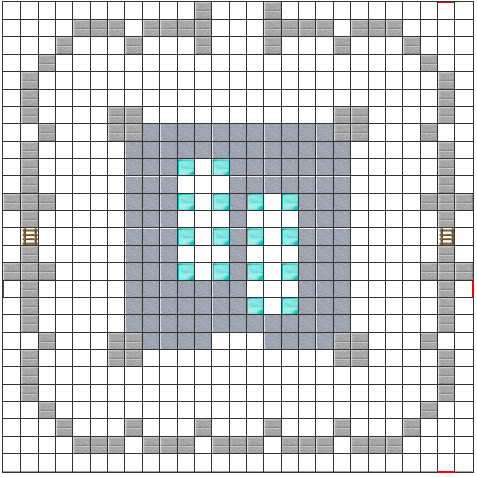
\includegraphics[width=0.7\textwidth]{qcraftblockrooms}
\caption{The floor plan for the rooms used to introduce the student to Observer Dependent Blocks, Quantum Blocks and entangled Quantum Blocks. The doors at the left and right side are only there in the Observer Dependency branch}
\label{fig:qcraftblockrooms}
\end{figure}

\begin{figure}[h!]
\centering
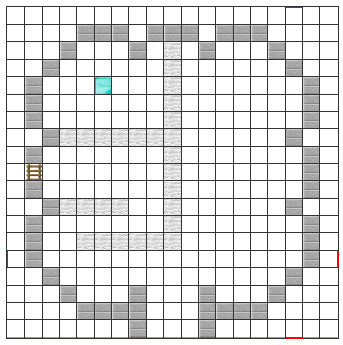
\includegraphics[width=0.5\textwidth]{odb-puzzle}
\caption{The floor plan of the puzzle within the Observer Dependency branch.}
\label{fig:odb-puzzle}
\end{figure}

\begin{figure}[h!]
\centering
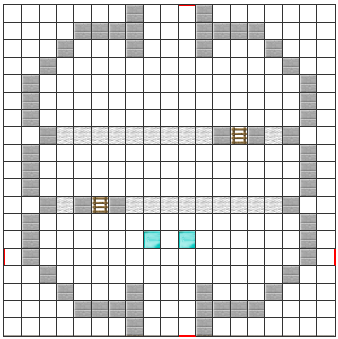
\includegraphics[width=0.5\textwidth]{qb-puzzle}
\caption{The floor plan of the first puzzle within the Quantum Block branch.}
\label{fig:qb-puzzle}
\end{figure}

\newpage

\section{The Evaluation Matchboard}
\label{app:evamatchboard}

\begin{figure}[h]
\centering
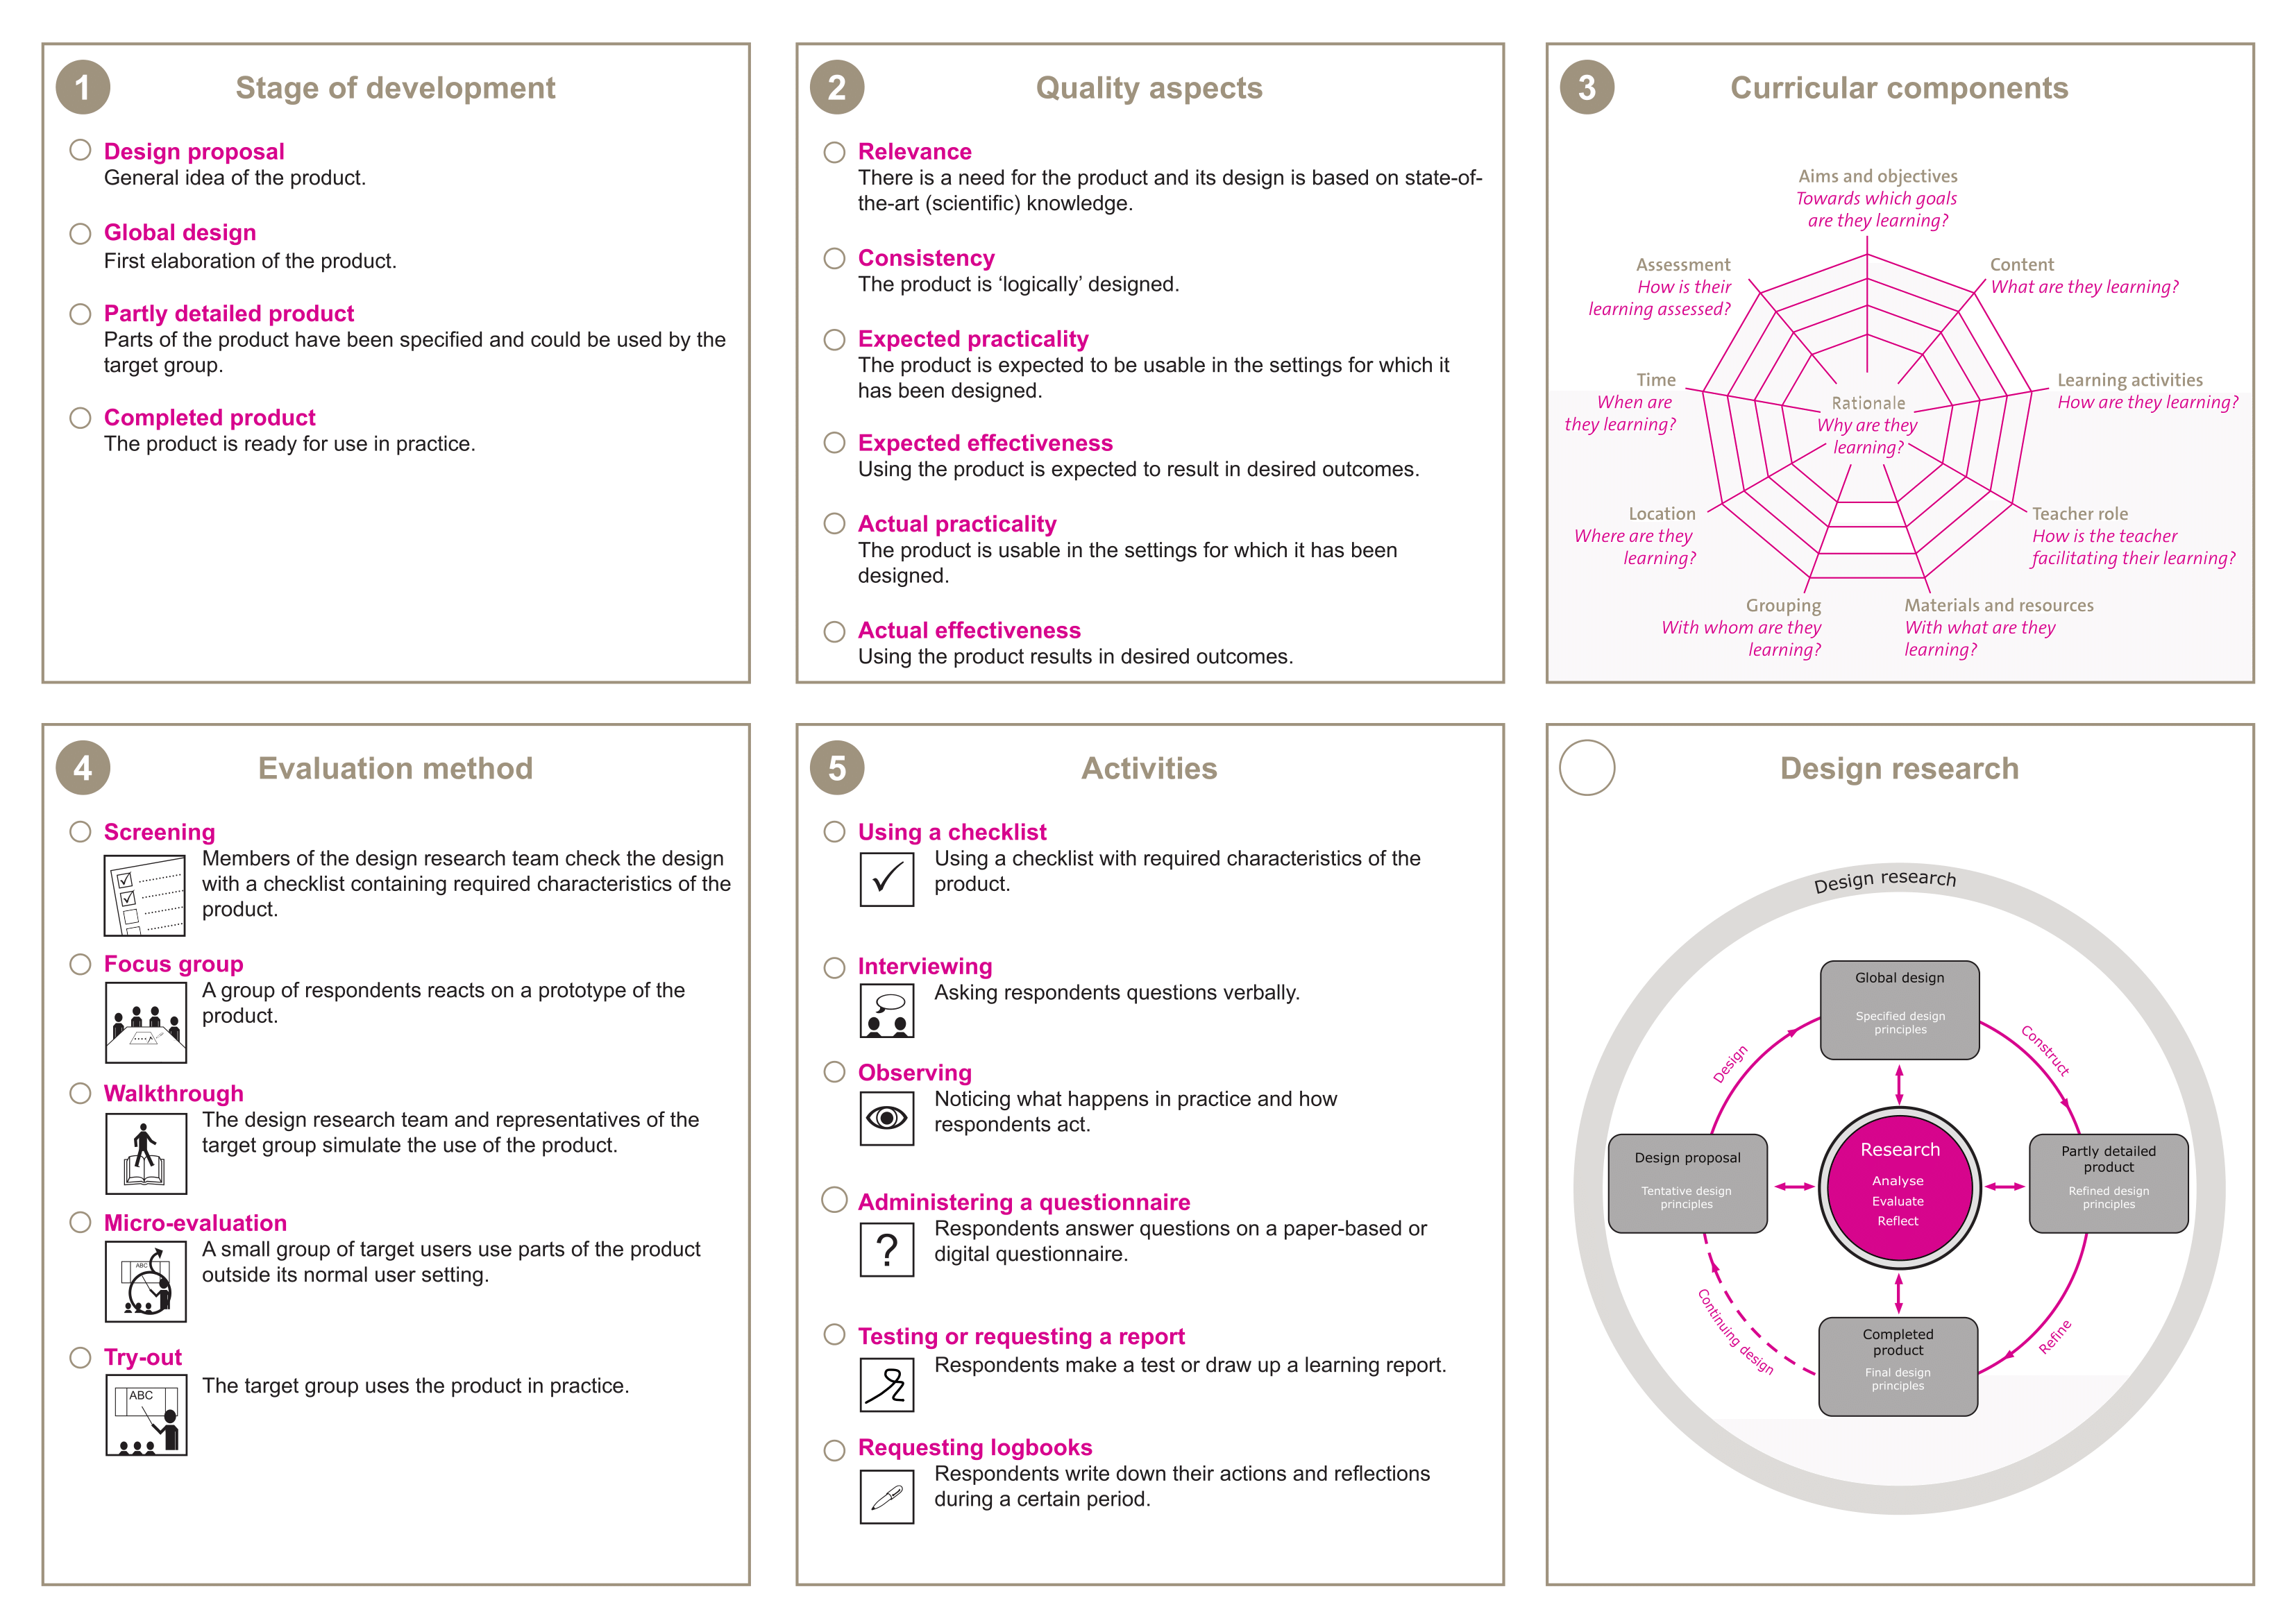
\includegraphics[angle=90, height=.75\textheight]{Evaluation_matchboard-1}
\end{figure}

\begin{figure}[h]
\centering
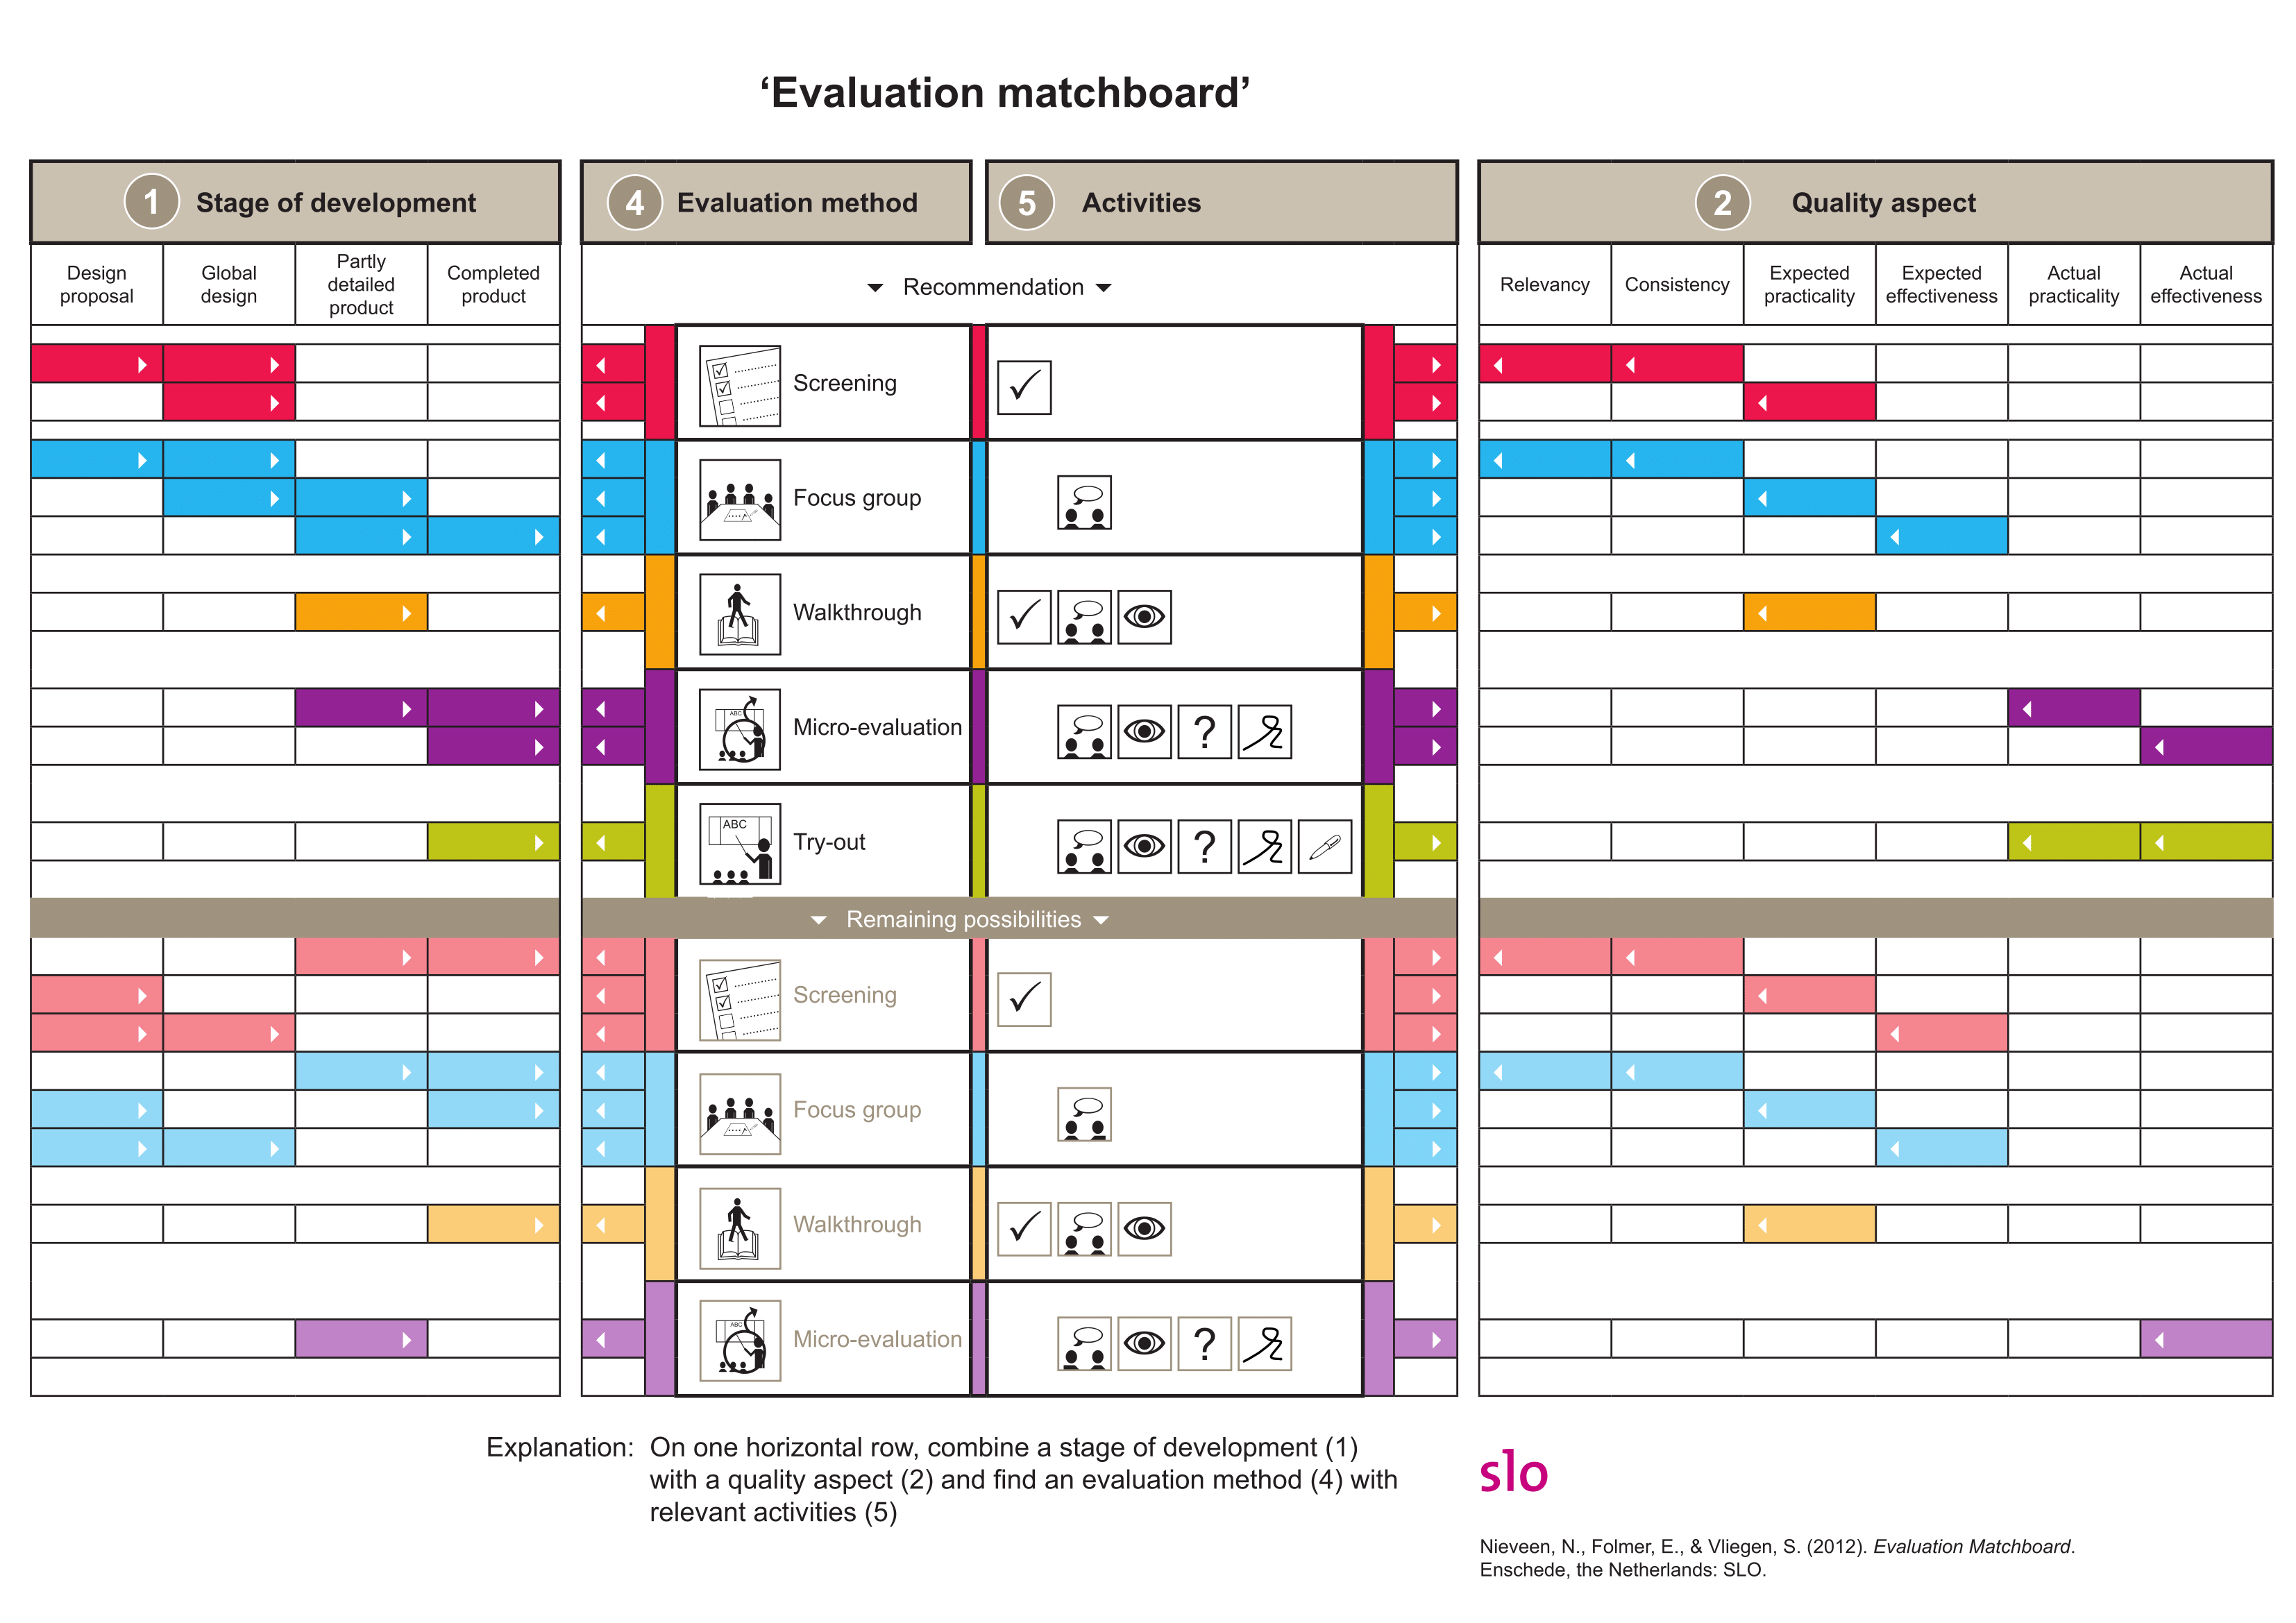
\includegraphics[angle=90, height=\textheight]{Evaluation_matchboard-2}
\end{figure}

\end{document}
